\documentclass[a4paper,11pt]{article}

\newcommand*{\cernroot}{\emph{ROOT}\xspace}
\newcommand*{\corry}{\emph{Corryvreckan}\xspace}
\newcommand*{\apx}{\emph{ATLASpix\_Simple}\xspace}
\newcommand*{\tpx}{\emph{Timepix3}\xspace}
\newcommand*{\module}[1]{\texttt{#1}}
\newcommand*{\code}[1]{\texttt{#1}}
\newcommand{\dir}[1]{\texttt{#1}}
\newcommand{\file}[1]{\texttt{#1}}


\newcommand{\gray}[1]{\textcolor{gray}{#1}}
\newcommand{\red}[1]{\textcolor{red}{#1}}

\usepackage[nottoc,numbib]{tocbibind}
% \usepackage{german}
\usepackage{amsmath}
\usepackage{amssymb}
\usepackage{graphicx,tabularx}
\usepackage[labelfont=bf]{caption}
\usepackage{subcaption}
\usepackage{epsf}
\usepackage{epsfig}
\usepackage{titlesec}
\usepackage{titletoc}
\usepackage{setspace}
\usepackage{bold-extra}
\usepackage{comment}
\usepackage{enumitem}
\usepackage{multicol}
\usepackage{float}
\usepackage{afterpage}
\usepackage{eurosym}
\usepackage[hang]{footmisc}
\usepackage{lipsum}
\usepackage{enumitem}
\usepackage{multirow}
\usepackage{booktabs}
\usepackage[T1]{fontenc}
\usepackage[utf8]{inputenc}
\usepackage{enumitem}
\usepackage{nicefrac}
\usepackage{color}
\usepackage[dvipsnames]{xcolor}
\usepackage{colortbl}
\usepackage{rotating}
\usepackage{xfrac}
%\usepackage{subfig}
\usepackage[rightcaption]{sidecap}
\sidecaptionvpos{figure}{c}
\usepackage[export]{adjustbox}
\usepackage[style=nature,autocite=superscript]{biblatex}% biblatex using nature style
%\usepackage[style=ieee,,dashed=false,autocite=superscript]{biblatex}% biblatex using IEEE style
%\usepackage[style=science,autocite=superscript]{biblatex}% biblatex using Science style
%\usepackage[biblatex=true,subcaption=true,default]{\ATLASLATEXPATH atlaspackage}% biblatex using ATLAS style
\usepackage[utf8]{inputenc}

\usepackage[amsmath,framed,thmmarks]{ntheorem}

\usepackage{afterpage}

\newcommand\blankpage{
	\null
	\thispagestyle{empty}
	\addtocounter{page}{-1}
	\newpage
}

\usepackage{hyperref}
\usepackage{siunitx}
\sisetup{range-phrase=--} % define -- as character for \SIrange{}{}
\sisetup{range-units=single}
\usepackage{makecell}

%% This stuff changes the font to sans serif - ugly but DFG "standard"
\usepackage{helvet}
\renewcommand{\familydefault}{\sfdefault}
%% End sans serif

\usepackage{xspace}

\newcounter{firstbib}
\newcounter{twobib}
\newcounter{diss}
\newcounter{temp}

\setlength{\topmargin}{-0,5cm}
\setlength{\textheight}{24cm}
\setlength{\textwidth}{17cm}
\setlength{\oddsidemargin}{-0.5cm}
\setlength{\evensidemargin}{1.5cm}
\setlength{\parindent}{0pt}
\setlength{\parskip}{7pt plus0.5pt minus0.5pt}

% Margins for item lists:
\setlist[itemize]{topsep=0pt, itemsep=0.5pt}

\newcommand\Tstrut{\rule{0pt}{2.6ex}}         % = `top' strut
\newcommand\Bstrut{\rule[-0.9ex]{0pt}{0pt}}   % = `bottom' strut

\setcounter{tocdepth}{2}
\sloppy
%\pagestyle{myheadings}

%\title{\boldmath GRK 1102 Physik an Hadron-Beschleunigern}


\hypersetup{
	% bookmarks=true,         % show bookmarks bar?
	unicode=false,          % non-Latin characters in Acrobat’s bookmarks
	pdftoolbar=true,        % show Acrobat’s toolbar?
	pdfmenubar=true,        % show Acrobat’s menu?
	pdffitwindow=false,     % window fit to page when opened
	pdfstartview={FitH},    % fits the width of the page to the window
	pdftitle={Characterisation of Silicon Pixel Sensors},% title
	pdfauthor={Jens Kr\"oger},     % author
	pdfsubject={Lab Course Manual, U Heidelberg},   % subject of the document
	pdfcreator={pdflatex},   % creator of the document
	pdfproducer={LaTeX with hyperref}, % producer of the document
	pdfkeywords={Particle Physics, Detector Development, Fortgeschrittenenpraktikum}, % list of keywords
	pdfnewwindow=true,      % links in new PDF window
	colorlinks=true ,       % false: boxed links; true: colored links
	linkcolor=blue,        % color of internal links (change box color with linkbordercolor)
	citecolor=green,        % color of links to bibliography
	filecolor=magenta,      % color of file links
	urlcolor=cyan           % color of external links
}


% your bibliographical database
\bibliography{references}

% path to figures:
\graphicspath{{figures/}}

\begin{document}

\begin{titlepage}

\begin{center}
\vspace{-4cm}
{\Huge \textbf{Solutions:}}\\
\vspace{1cm}
{\Huge {Characterisation of Silicon Pixel Sensors}}\\
\vspace{1cm}
{\Huge {for High-Energy Physics \gray{and beyond}}}

\vspace{0.7cm}
{\large \textbf{\red{Only for Tutors}}}\\
\vspace{0.3cm}
{\large Version 1.0.2 (\today)}

\vspace{1cm}

\fbox{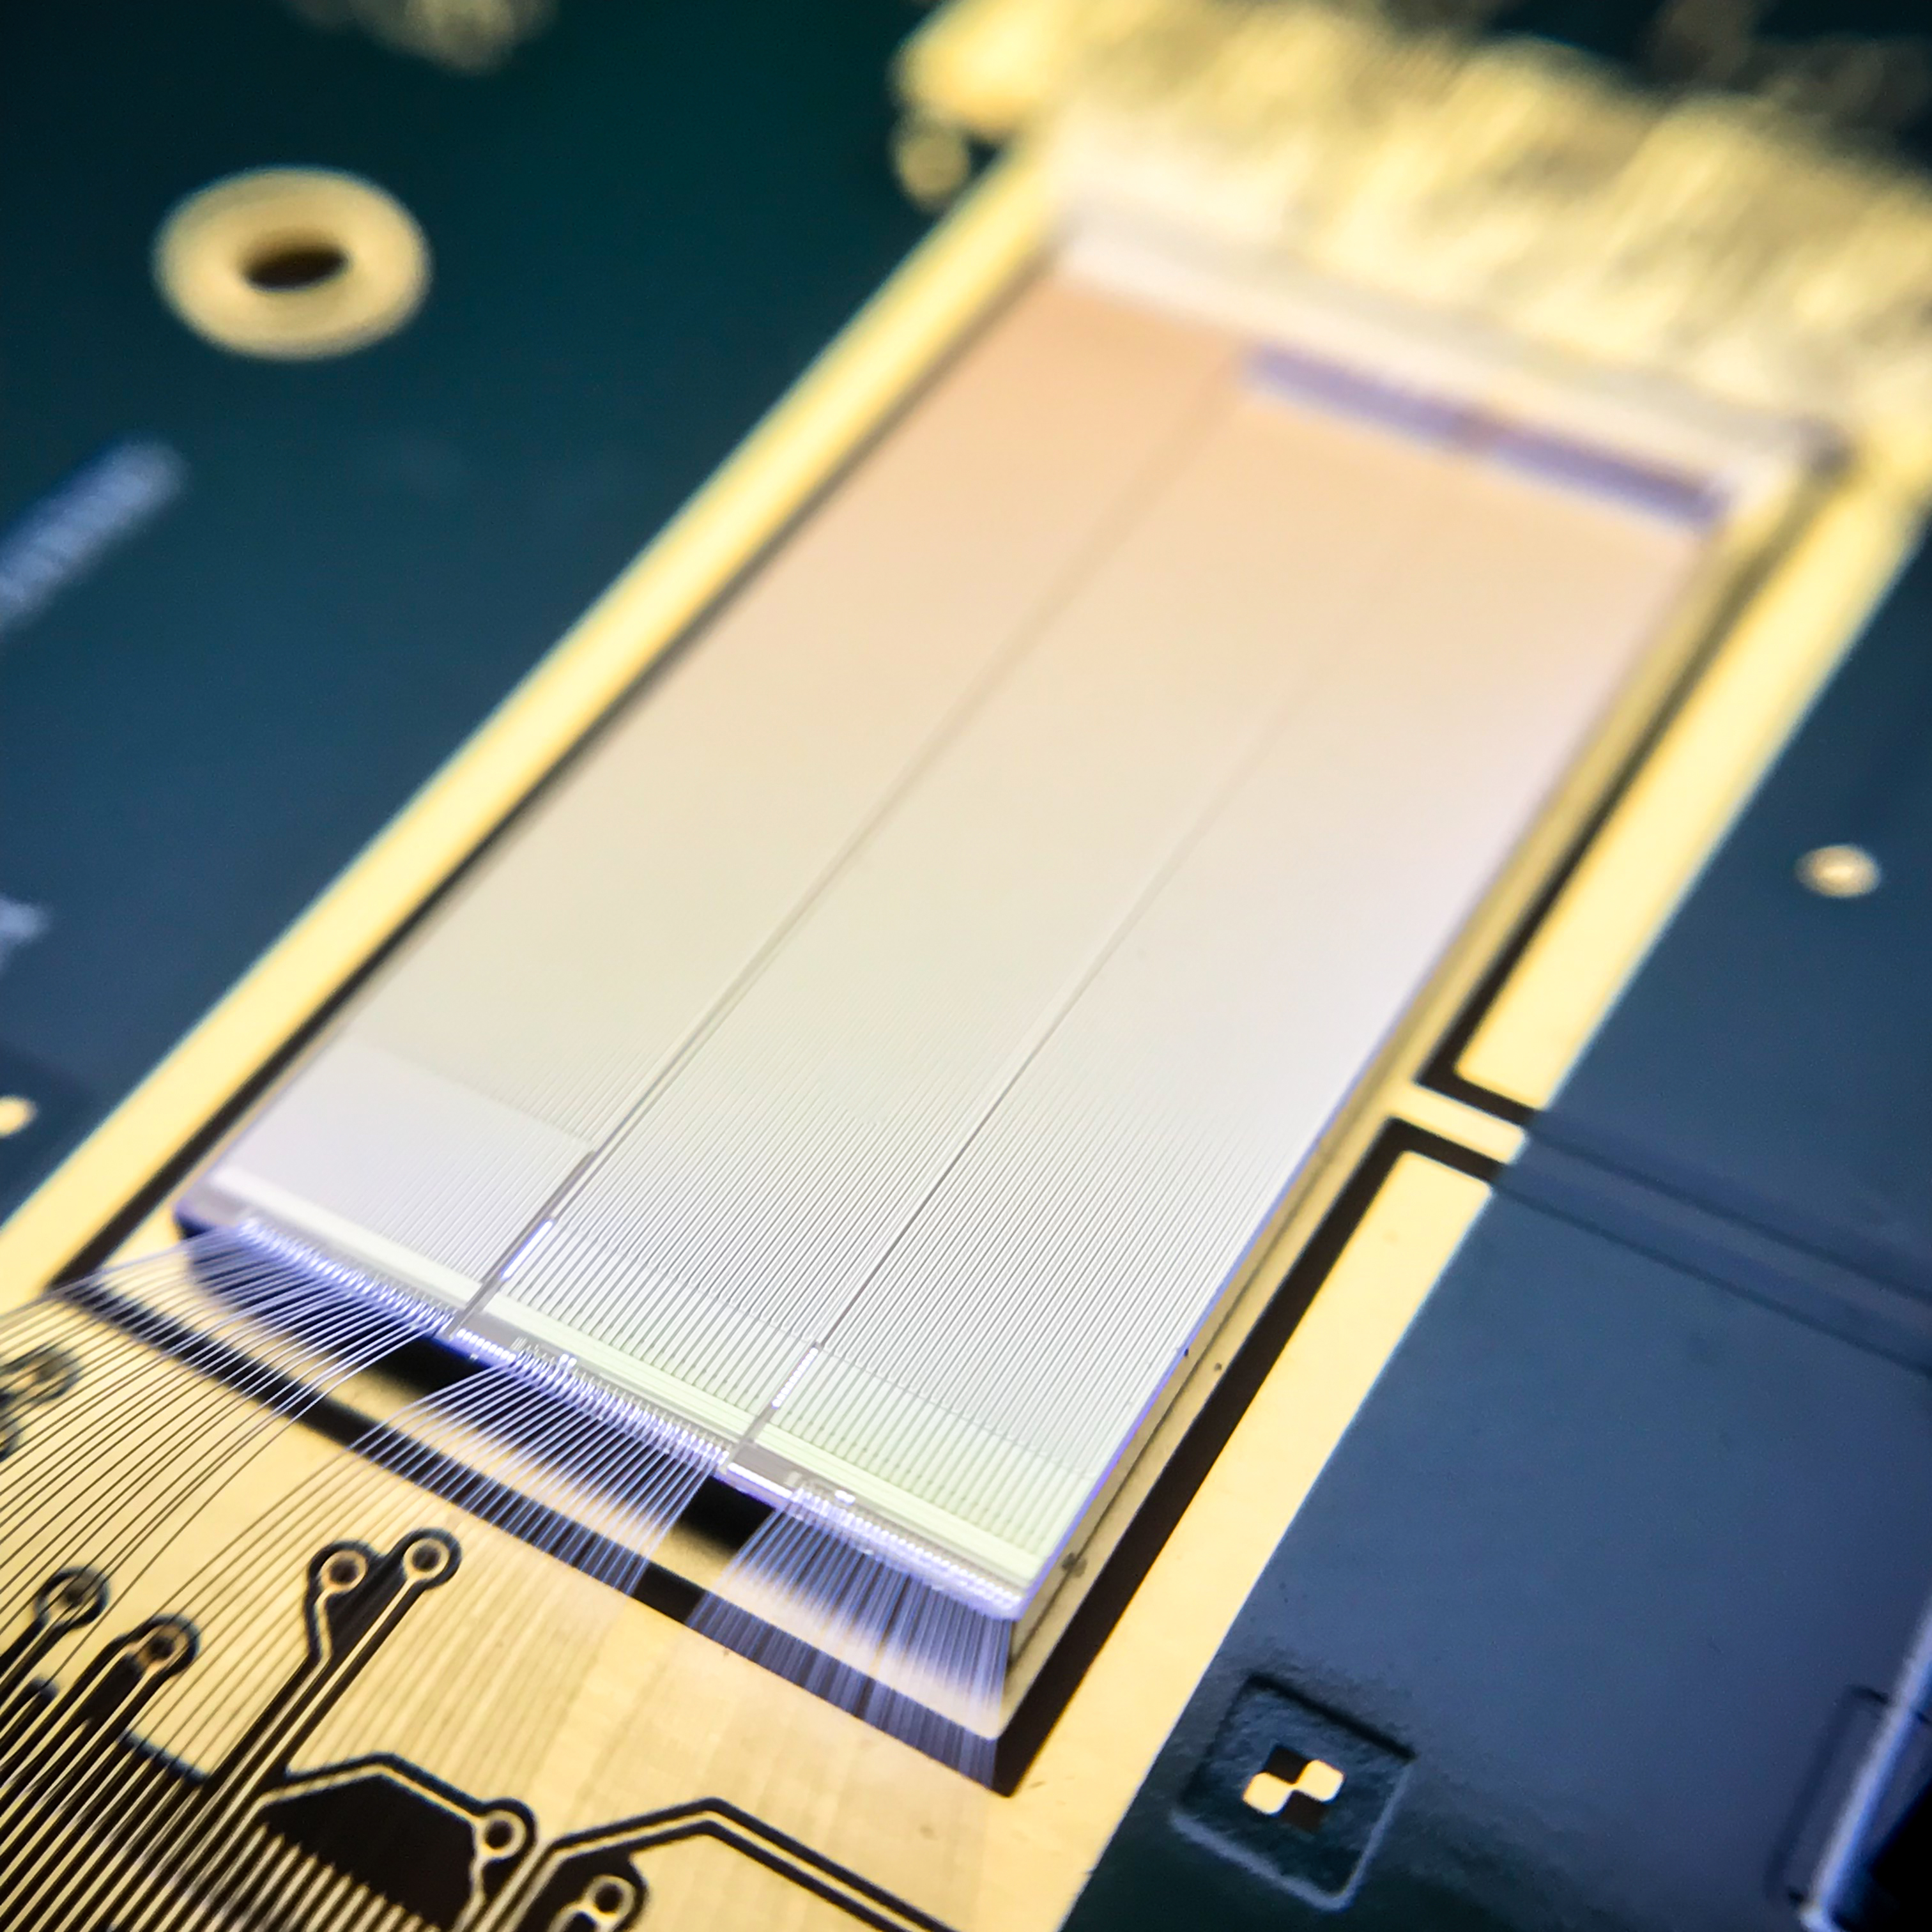
\includegraphics[width=.66\textwidth]{figures/ATLASpix_photo.jpg}}

\vspace{2.cm}
{\large \textbf{Author:} Jens Kr\"oger\\[0.3cm]}
{\large \textbf{Contact:} jens.kroeger@cern.ch }

\vspace*{\fill}
\large{\textbf{Fortgeschrittenen-Praktikum (FP)}\\}
\large{Universit\"at Heidelberg\\}

\end{center}
\afterpage{\blankpage}

\end{titlepage}

\tableofcontents
\clearpage

\section{Brief Overview}
The repository with the templates and configuration files for this lab course can be found here:\\
\url{https://gitlab.cern.ch/jekroege/fp_pixel_sensor_characterisation}

\textbf{Important:} Note that the git repo contains two branches:
\begin{itemize}
\item \code{for\_students}: contains all the 'empty' templates for the students to fill out during the lab course.
This branch is \textbf{checked out by default} so the students won't know notice unless they know how to use git.
\item \code{master}: This branch contains the same templates as above but in addition also fully functional configuration files and the final geometry file with a good alignment.
\end{itemize}

The repository with the LaTeX source code and all figures for both the manual and this document with solutions can be found here:\\
\url{https://gitlab.cern.ch/jekroege/fp_manual/}

\section{Introduction and Theory}

\subsection{Silicon Pixel Sensors}

\subsubsection{Semiconductor Physics}
All questions can be answered with basic textbook knowledge.

\subsubsection{Interaction of Particles with Matter}
All questions can be answered with basic textbook knowledge.

\subsubsection{Silicon Pixel Sensors}
\begin{itemize}
\item \textbf{How is a signal generated in a pixel sensor?}\\
An ionising particle passing through the sensor creates electron-hole pairs.
If these are created outside of the depleted volume of the sensor, they diffuse in random directions.
Either they recombine after a while or they diffuse into the depletion region, where they are accelerated towards the collection electrode by the electric field of the diode.
The same happens for electron-hole pairs that are created inside the depleted region.
\textbf{Important:} The measured signal corresponds to the signal induced on the collection electrode by the moving charges (Shockley Ramo theorem) and not the collected charges themselves.
It is therefore earlier and has the opposite charge of the collected charges.
The signal is then amplified and discriminated in a comparator.
\item \textbf{What is a ToT measurement and how can it be translated into energy?}\\
The time-over-threshold (ToT) is the time a given signal is higher than the threshold of the comparator.
A signal corresponding to a large amount of deposited energy is larger because more electron-hole pairs are created. 
Consequently, the ToT is larger in this case.
The ToT can be translated into signal charge.
For this, a calibration is needed, in which photons with a well-defined energy (from radioactive sources or X-ray tubes) are used to measure which pulse height (and thus which ToT) corresponds to which charge.
\item \textbf{Which spectrum is expected for energy loss of ionising particles in thin layers? What does this have to do with the time-over-threshold?}\\
The energy loss (deposited charge) by MIPs in thin layers follows a Landau distribution -- this can also be found in the recommended textbook.
Consequently, the measurement of the charge spectrum by means of the ToT can be described by a Landau convoluted with a Gaussian due to the wash-out of the measurement by fluctuations of the detection threshold.
\item \textbf{What is noise? What can cause it?}\\
Noise refers to pixels that record a hit, i.e.~its signal exceeds the comparator threshold without an ionising particle passing through.
It can be caused by (thermal) fluctuations of the amplifier output signal or the detection threshold of the comparator.
\end{itemize}

\subsubsection{Hybrid Sensors}
Questions combined with next section.

\subsubsection{Monolithic Pixel Sensors}
\begin{itemize}
\item \textbf{What is the difference between hybrid and monolithic detectors? Can you think of advantages and disadvantages of the two technologies?}
\end{itemize}

\textbf{Hybrid Sensors:}
\begin{itemize}
\item[+] Sensor and readout electronics can be developed separately.
\item[+] Readout electronics can be reused for different sensors.
\item[+] High electric field in sensor is well separated from sensitive electronics of readout chip.
\item[-] Bump bonding is expensive.
\item[-] The bump bonds limit the achievable minimal pixel pitch (\SI{\sim25}{\micro m}).
\end{itemize}
\textbf{Monolithic Sensors:}
\begin{itemize}
\item[+] Based on commercially available (imaging) manufacturing processes\\ $\rightarrow$~reduced cost and manufacturing complexity
\item[+] No bump bonding $\rightarrow$~cheaper, better for mass production
\item[+] Sensors can be thinned $\rightarrow$~very low material budget (thickness)
\item[-] Possible influence of the sensor on the electronic circuitry and vice versa
\item[-] complex sensor layouts and limited information on processing details (which is needed for simulations)
\end{itemize}

\subsubsection{Sensor Characterisation}
No questions.

\subsubsection{Test-Beam Facilities}
No questions.

\subsubsection{The Reference Telescope}
No questions.

\subsubsection{The Device-under-Test}
No questions.

\section{Basics of Test-beam Analysis}
This section is supposed to give an overview ('global picture') and explain some of the basics.
If the students do not yet understand all the concepts, that's no problem. 
Many things will be much easier to understand when performing the analysis and seeing the output histograms.

\textbf{Important:} In many cases, the answers to questions in Section~\ref{sec:instructions} can be found here, so encourage the students to read it again as they go through the analysis instructions.

\subsection{Overview of the Software}
No questions.

\subsection{The Test-beam Reconstruction Chain}
No questions.

\section{Instructions}
\label{sec:instructions}

\subsection{Getting Familiar with the Tools}
No questions.

\textbf{Note:} If the students observe that their histogram names don't comply with the manual and they installed \corry on their own PC, they might not have checked out the correct \corry branch \code{fp\_heidelberg}.
If they compiled the latest master and then switch to \code{fp\_manual}, they will need to delete the \code{bin/}, \code{build/} and \code{lib/} directories and re-compile to avoid conflicts.

\subsection{Reading in the Raw Data}
See Figure~\ref{fig:02_hitmaps}.
\begin{itemize}
\item \textbf{Do you see a pattern? Can you explain it?}\\
The observed pattern corresponds to the beam spot.
The beam has a gaussian profile and is more intense in the center.
Consequently, there are more hits in the center.
\item \textbf{Does any of the telescope planes look significantly different from the others? What might cause it?}\\
The hitmap of the \code{Timepix3\_4} looks different.
By zooming into the z-axis it can be seen that this is due to a noisy pixel in the bottom left.
This shifts the range of the z-axis which makes the histogram appear different.
By setting it to a similar range compared to the other hitmaps, the pattern of the beam spot looks the same.
The noisy pixel(s) could be masked for the following analysis.
However, the influence on the final results is negligible.
\end{itemize}

\begin{figure}[!htb]
\centering
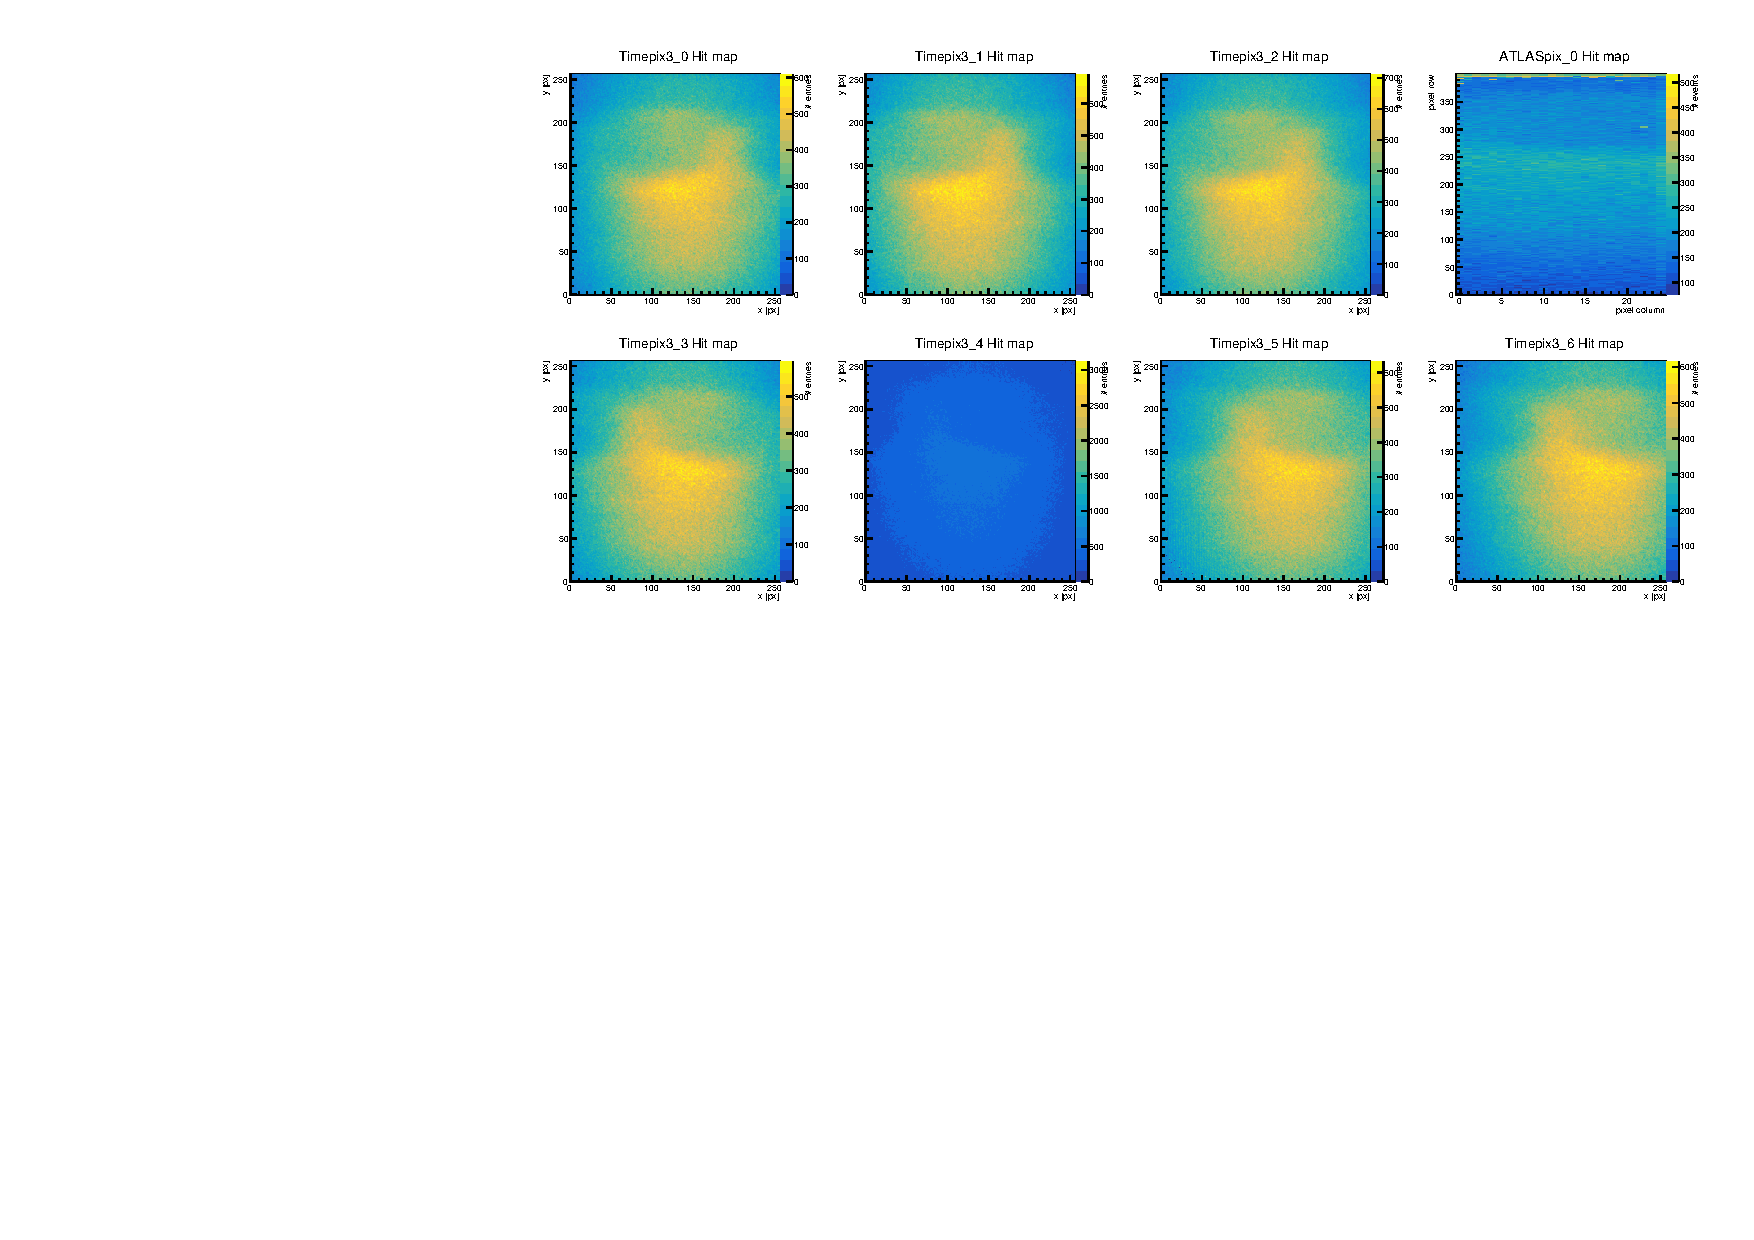
\includegraphics[width=\textwidth]{02_read_data_hitmaps}
\caption{Hitmaps of all \tpx telescope planes and the \apx.}
\label{fig:02_hitmaps}
\end{figure}

\subsection{Clustering}
See Figure~\ref{fig:03_clustering}.
\begin{itemize}
\item \textbf{Compare the cluster sizes for the \tpx and the \apx. How do they differ? Why?}\\
The average cluster size on the \tpx is much larger (peak at \SI{\sim4}{}) than for the \apx (peak at \SI{\sim1}{}).
This can be explained because the \tpx has much more charge sharing for two reasons:
Firstly, the detector design is different: the sensor layer is much thicker leading to much more lateral diffusion. Secondly, the \tpx is rotated by \SI{9}{\degree}, which increases the charge sharing as the traversing particles are likely to pass through more than one pixel.
\item \textbf{Compare the cluster width in column and row for the \apx. How do they differ? Why?}\\
The cluster widths in column in row are very similar.
However, the cluster width in column direction is slightly smaller than in row direction.
This coincides with the pixel dimensions: There is (even) less charge sharing along the columns, which have a pitch of \SI{130}{\micro m} compared to the rows with a pitch of \SI{40}{\micro m}.
\item \textbf{Compare the seed pixel ToT and the cluster ToT for the \apx (for the \tpx). Which difference can you observe for the \apx and the \tpx? Why?}\\
In case of the \apx, the pixel ToT and the cluster ToT distribution are very similar. That's because there are mostly single-pixel clusters (see previous question).
In contrast, the cluster ToT for the \tpx is much larger than the seed pixel ToT because there are mostly multi-pixel clusters, i.e.~the seed pixel only contains a smaller fraction of the total cluster charge.
\end{itemize}

\begin{figure}[!htb]
\centering
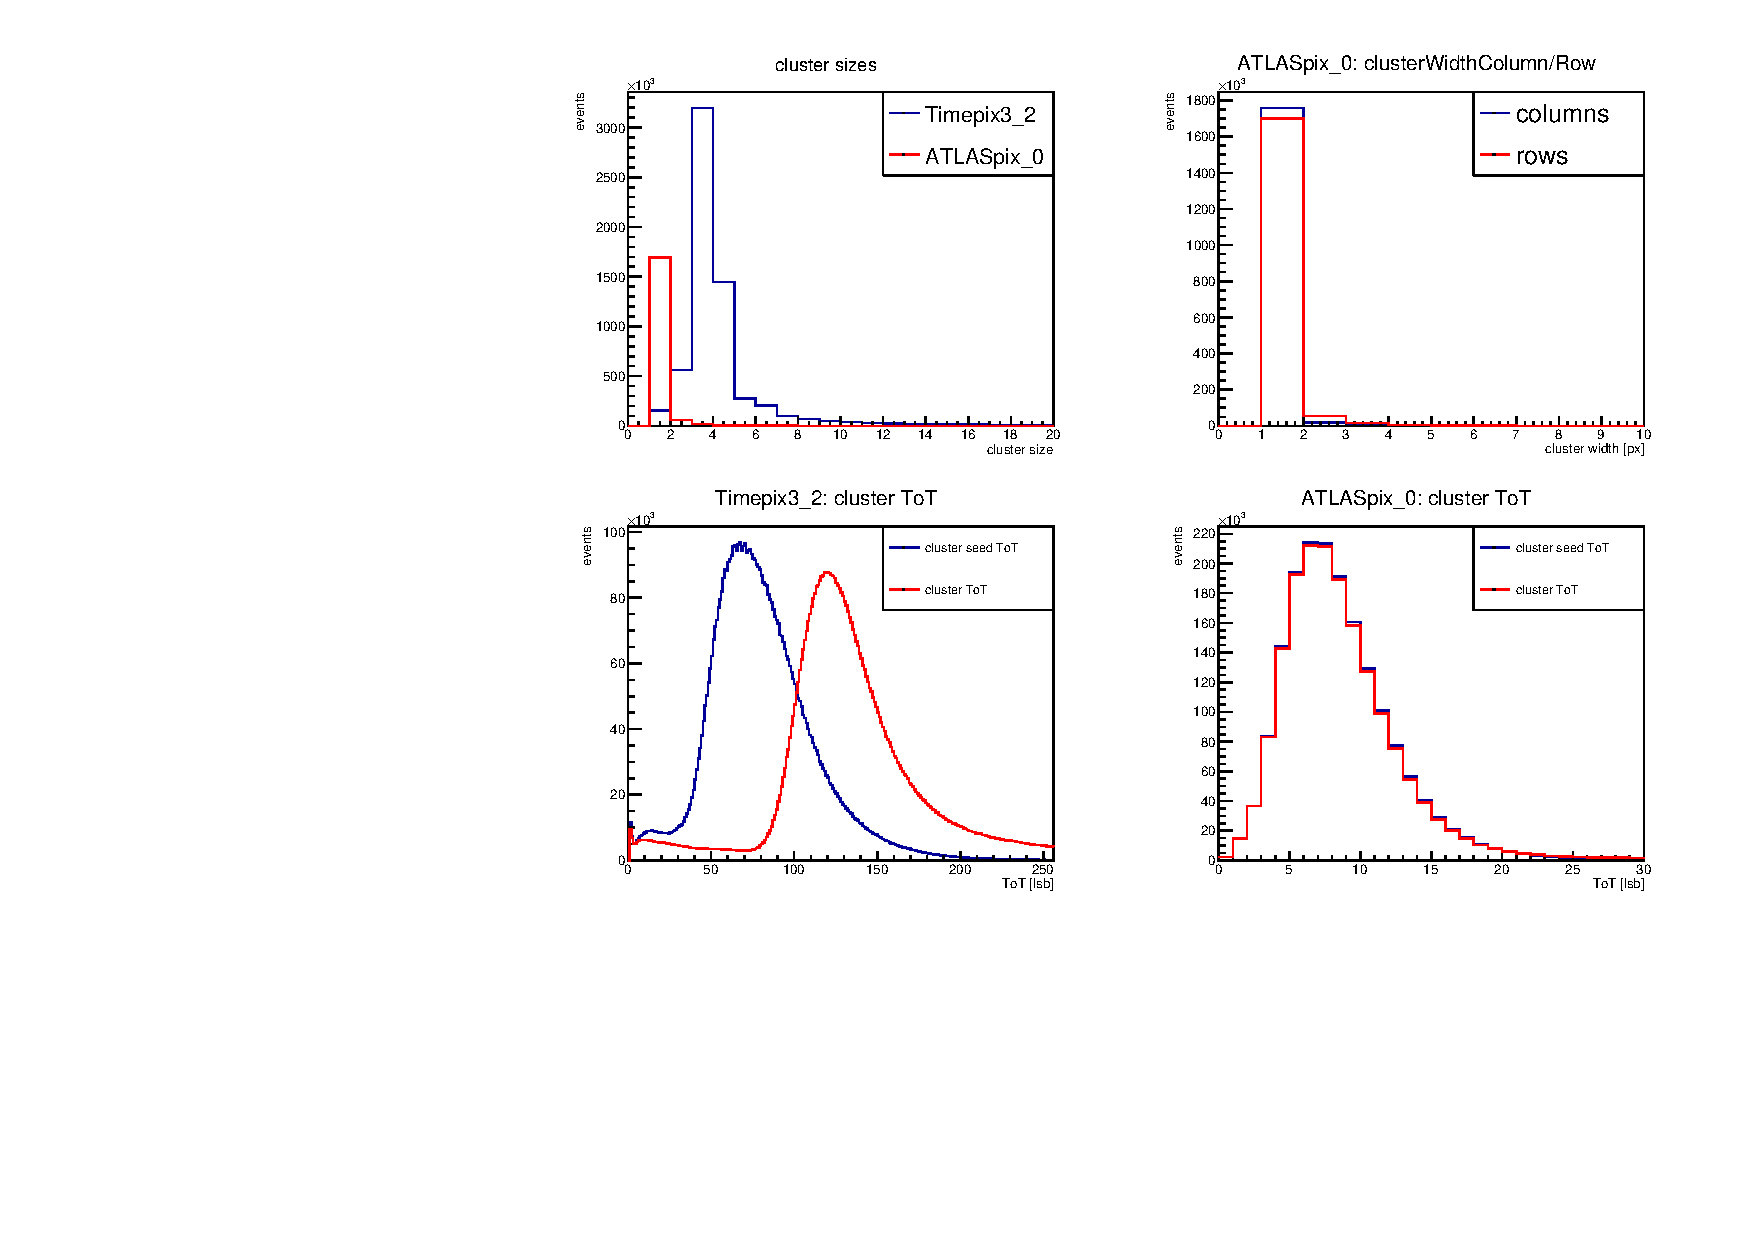
\includegraphics[width=\textwidth]{03_clustering}
\caption{Cluster Sizes and ToT distributions.}
\label{fig:03_clustering}
\end{figure}

\subsection{Correlations}
The students don't need to write a \cernroot macro here.
It's enough to inspect the \cernroot file with the \code{TBrowser} and give qualitative answers.
\begin{itemize}
\item \textbf{How can translational misalignments be observed in the correlations? How large are they approximately in your case? How many pixel pitches do they correspond to?}\\
A translational misalignment can be seen in an offset of the peak from zero. If this shift is $\mathcal{O}($\SI{200}{\micro m}), this already corresponds to multiple pixel pitches.
This can be tested easily but re-running the analysis with an added translational misalignment of \SI{\pm200}{\micro m} (as an example).
\item \textbf{How can a bad rotational alignment be observed in the correlations?}\\
A bad rotational alignment makes the peak of the correlations much broader.
This can be tested easily but re-running the analysis with a rotational misalignment of \SI{\pm20}{\degree} (as an example).
\end{itemize}

\subsection{Alignment and Tracking}

\subsubsection{Prealignment}
See Figure~\ref{fig:05_prealignment}.
\begin{itemize}
\item \textbf{Divided canvas with the correlations in y for all \tpx planes before and after the prealignment to show that they are centered at zero now.}\\
It can be seen that the correlations are shifted towards zero during the prealignment. Their widths are unchanged because we did not change the rotations specified in the geomety file.
The correlations of the reference plane appear very sharp as they show a self-correlation.
\end{itemize}

\begin{figure}[!htb]
\begin{subfigure}{\textwidth}
\centering
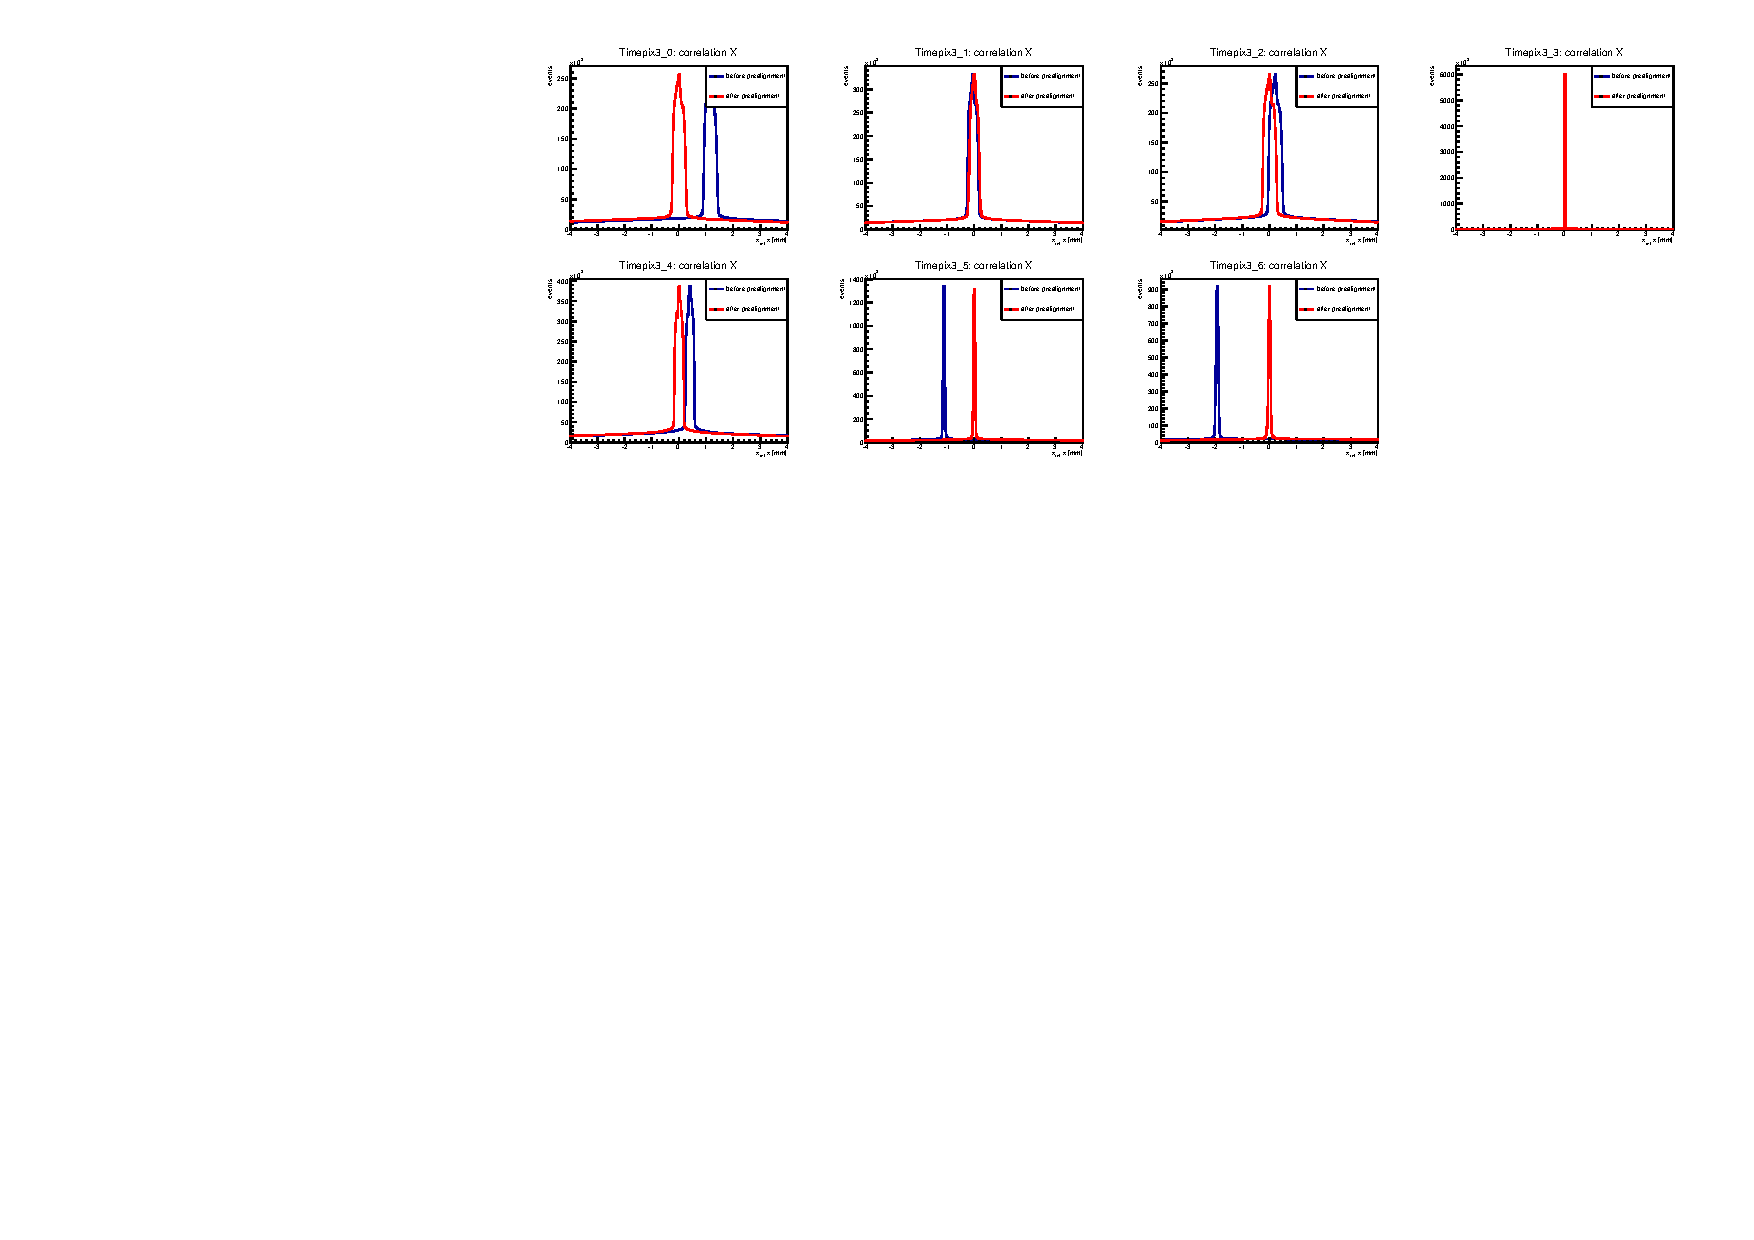
\includegraphics[width=\textwidth]{05_prealignment_X}
\caption{Correlations in x.}
\label{fig:05_prealignment_X}
\end{subfigure}
\begin{subfigure}{\textwidth}
\centering
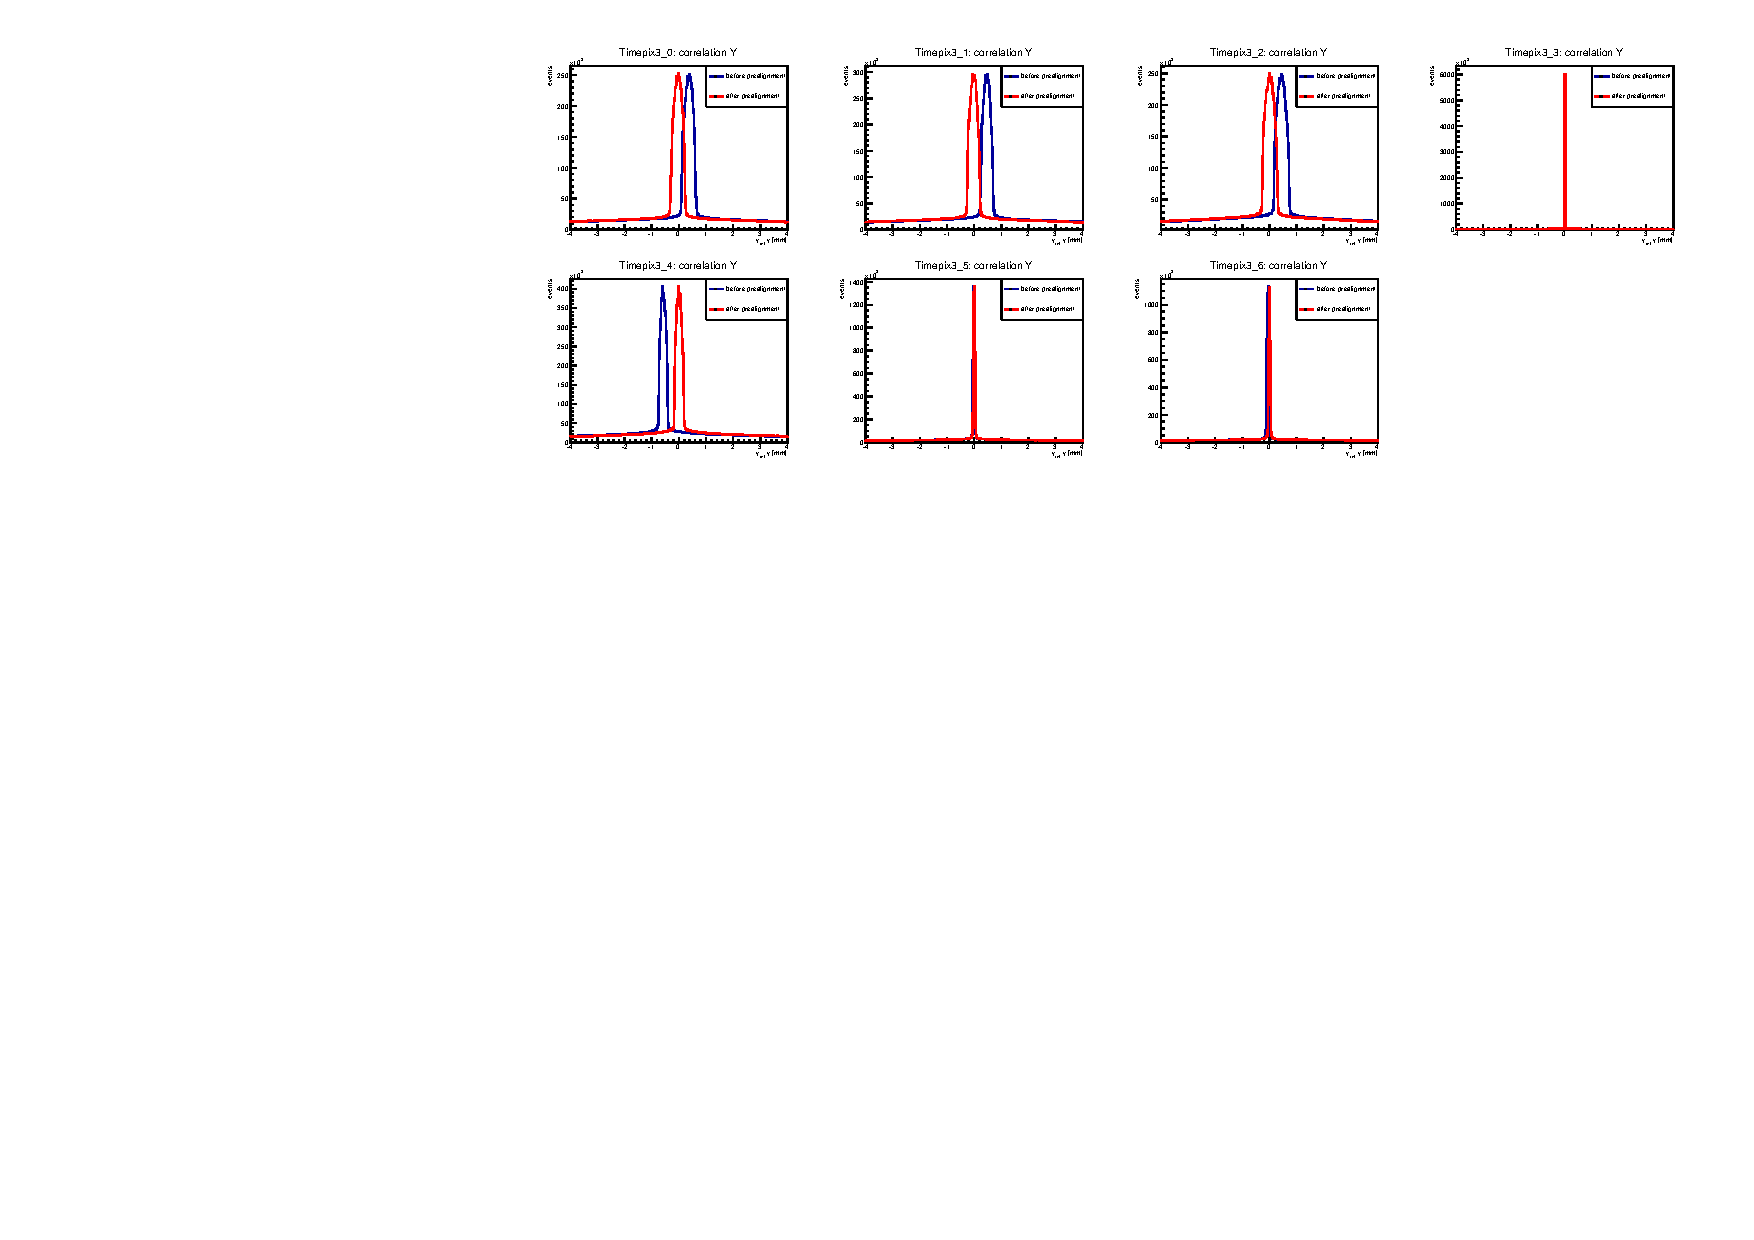
\includegraphics[width=\textwidth]{05_prealignment_Y}
\caption{Correlations in y.}
\label{fig:05_prealignment_Y}
\end{subfigure}
\caption{Correlations for all \tpx before and after performing the prealignment.}
\label{fig:05_prealignment}
\end{figure}

\newpage
\subsubsection{First Tracking}
See Figure~\ref{fig:06_first_tracking}.
The students don't need to write a \cernroot macro here.
It's enough to inspect the \cernroot file with the \code{TBrowser} and give qualitative answers.
\begin{itemize}
\item \textbf{Compare the residuals with the correlations from the previous analysis. What is the difference?}\\
Both the correlations and the residuals are somewhat centered around zero.
However, the residual histograms have only very few entries.
This is because the alignment is still too bad for good tracking results, i.e.~not many tracks were found.
\item \textbf{As you remember, a reasonable fit should have a $\chi^2/\text{ndof} \sim 1$.
What does the track $\chi^2/\text{ndof}$ look like for you? Why?}\\
It can be seen that most entries end up in the overflow bin.
This supports the previous observation that the alignment is not good enough for the tracking to work well.
\end{itemize}

\begin{figure}[!htb]
\centering
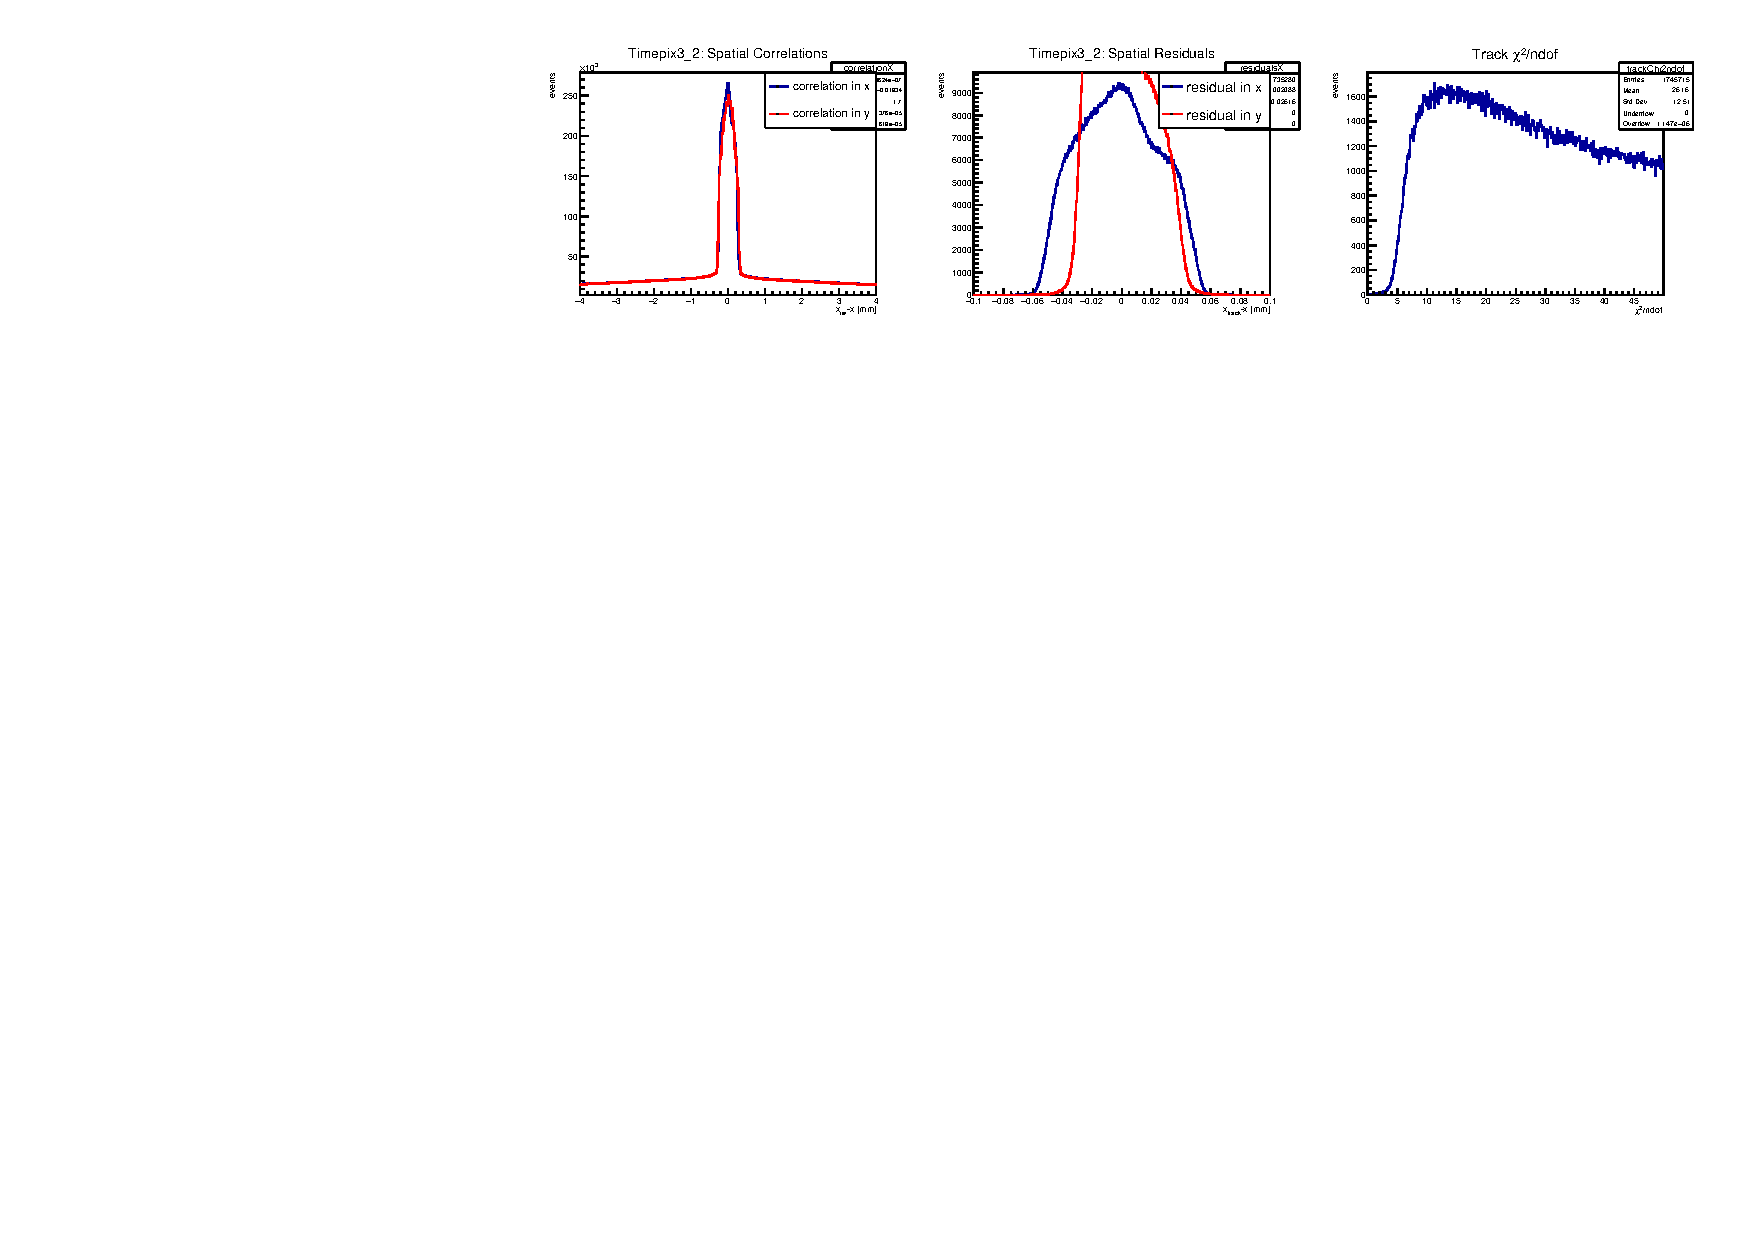
\includegraphics[width=\textwidth]{06_first_tracking}
\caption{Correlations and residuals in x and y for the \code{Timepix3\_2}, and track $\chi^2/\text{ndof}$ after performing the prealignment.}
\label{fig:06_first_tracking}
\end{figure}

\subsubsection{Telescope Alignment}
\textbf{Note:} It should suffice to run the alignment with the suggested settings \textbf{once} to achieve a reasonable alignment.
If the alignment doesn't work well, most likely a parameter was set wrongly or the prealignment was not good enough.
See Figure~\ref{fig:07_alignment}.
\begin{itemize}
\item \textbf{Overlay the $\chi^2/\text{ndof}$ distributions before and after the alignment. Explain what you see.}\\
Before the alignment, nearly all entries end up in the overflow bin of the histogram.
After the alignment, the distribution peaks at one, which means that the majority of track fits have a good $\chi^2$ and are therefore usable for the further analysis.
\item \textbf{Divided canvas with the residuals in x and y for all \tpx planes before and after the alignment.}\\
The residuals before the alignment are hardly filled because not many tracks were found.
After the alignment, the residuals are nicely centered at zero and more narrow than previously.
\end{itemize}

\begin{figure}[!htb]
\begin{subfigure}{\textwidth}
\centering
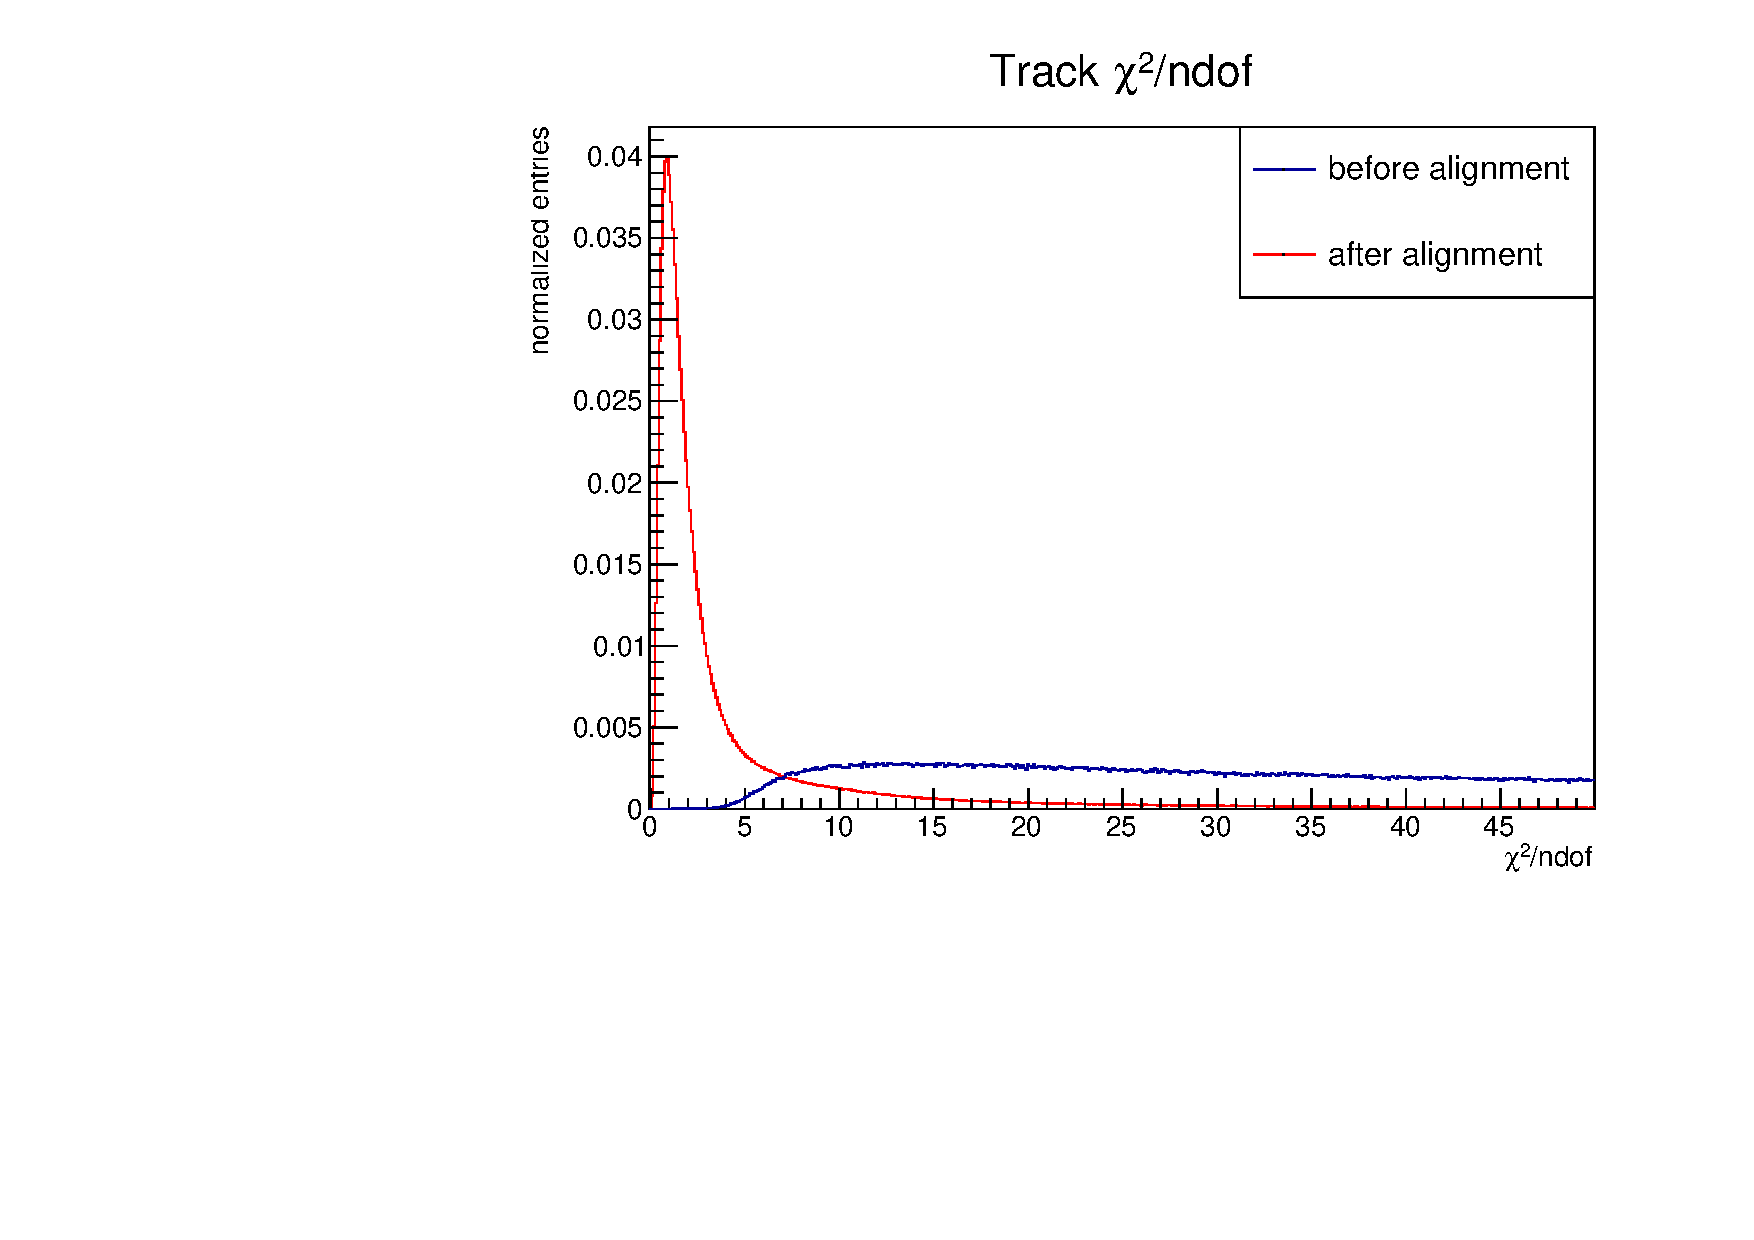
\includegraphics[width=0.45\textwidth]{07_alignment_trackChi2}
\caption{Track $\chi^2/\text{ndof}$.}
\label{fig:07_alignment_trackChi2}
\end{subfigure}
\begin{subfigure}{\textwidth}
\centering
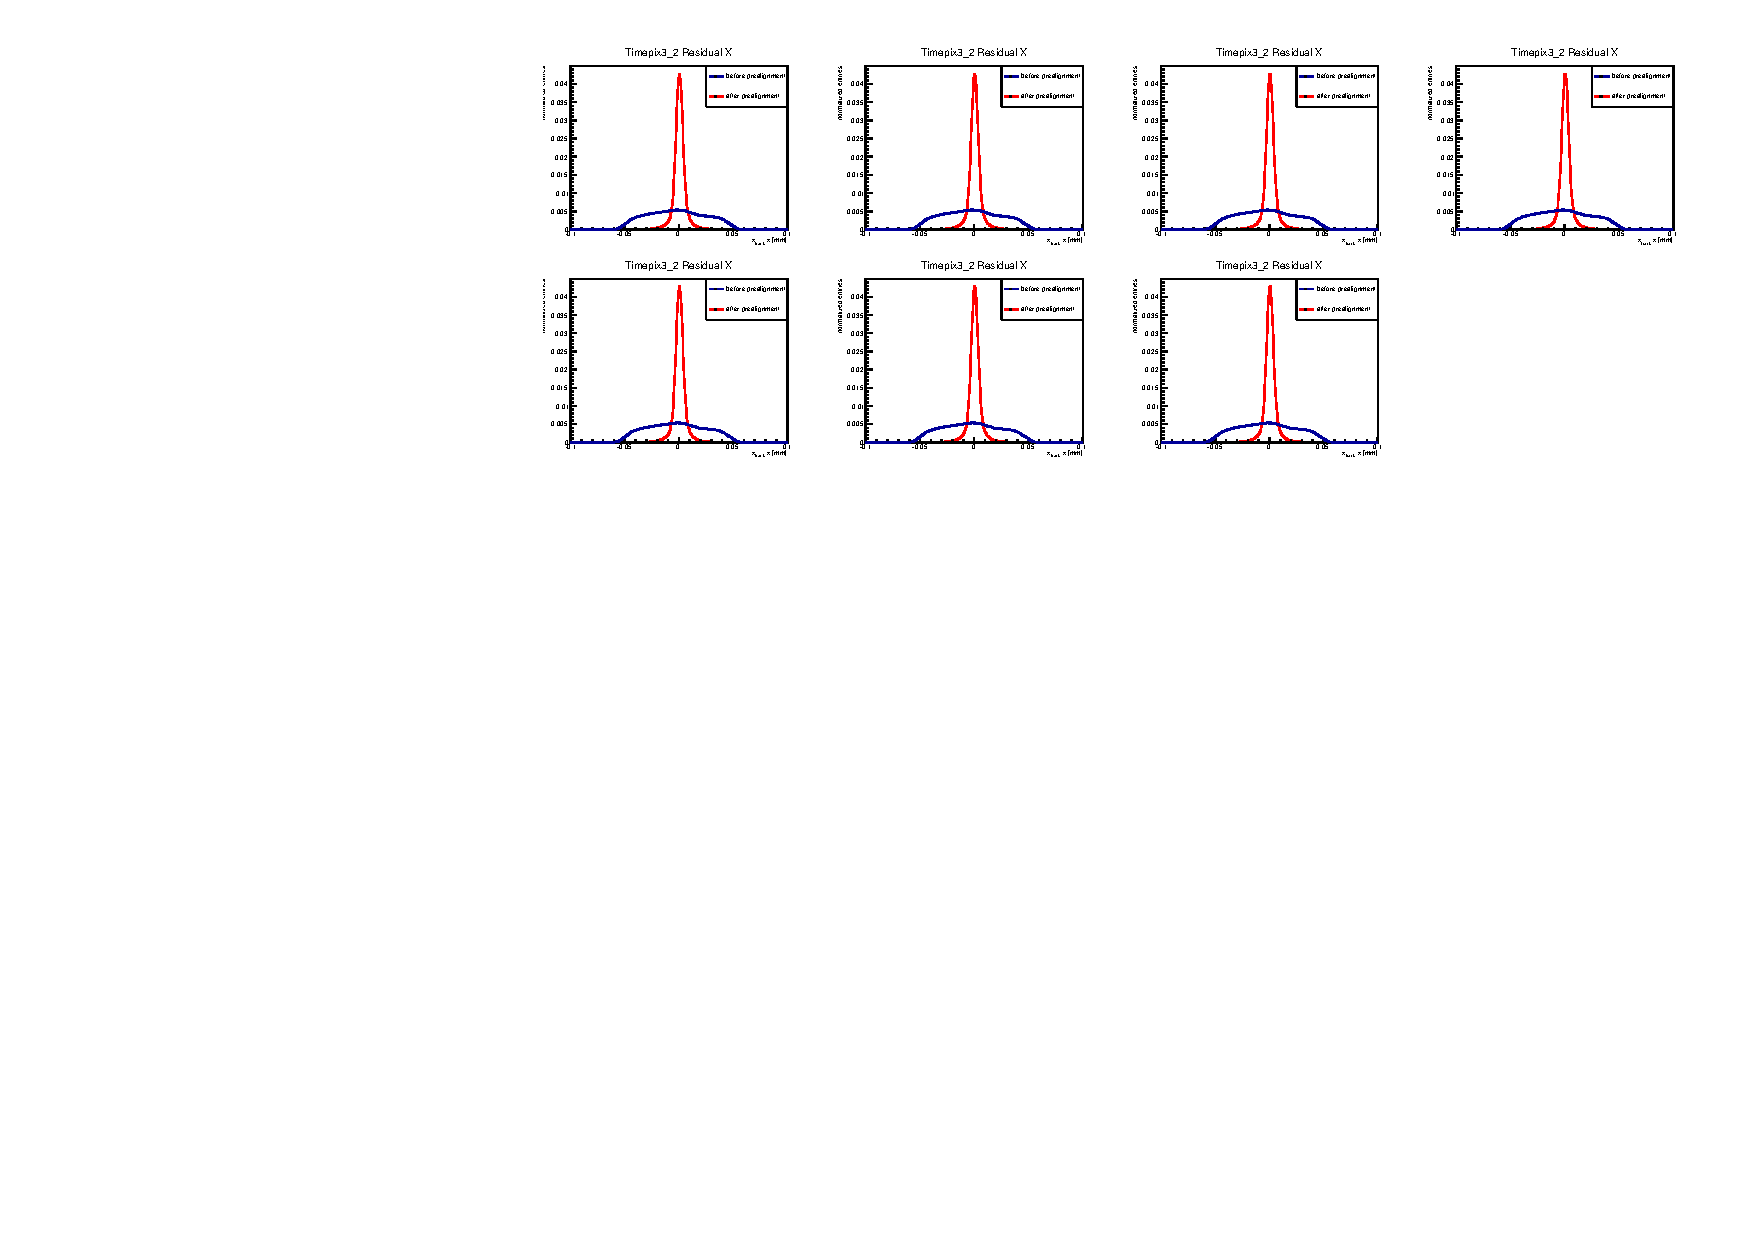
\includegraphics[width=\textwidth]{07_alignment_residualsX}
\caption{Spatial residuals in x.}
\label{fig:07_alignment_X}
\end{subfigure}
\begin{subfigure}{\textwidth}
\centering
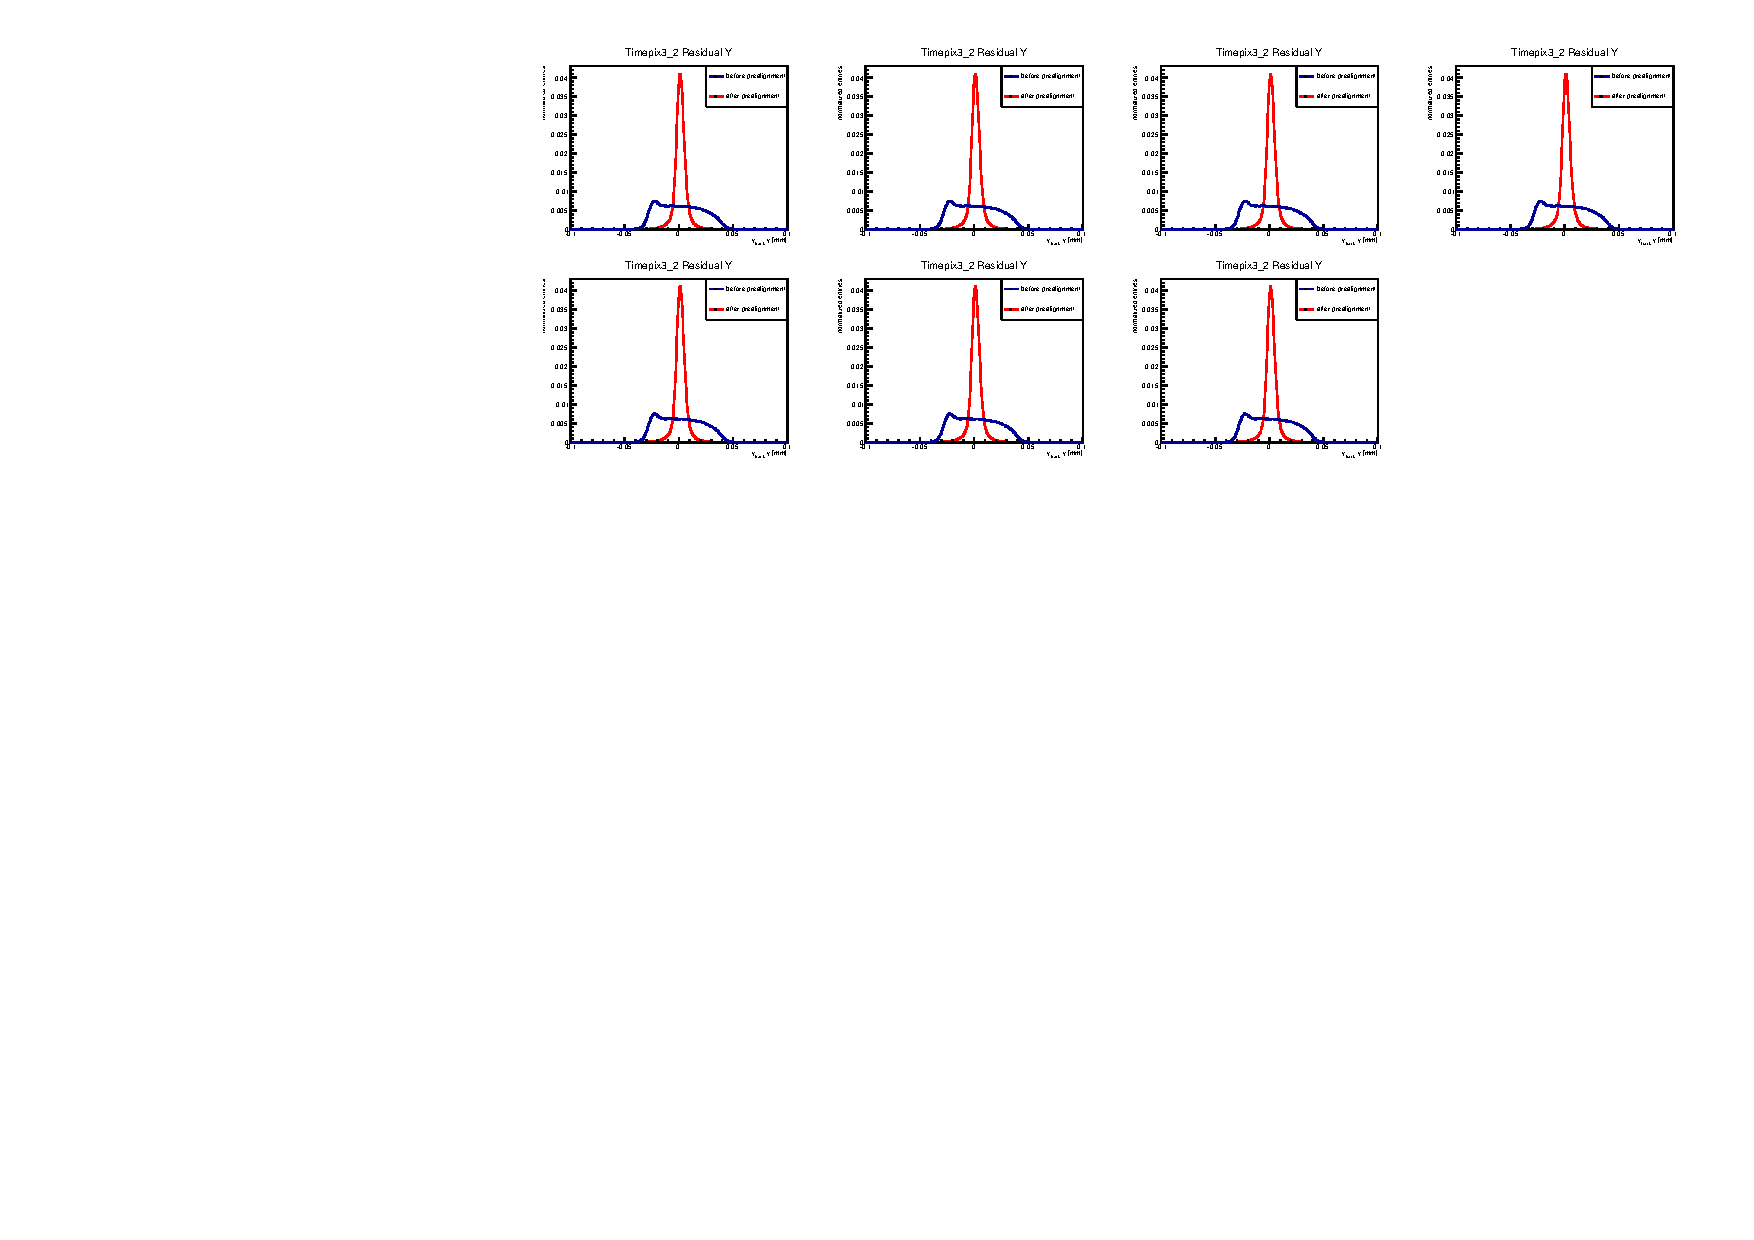
\includegraphics[width=\textwidth]{07_alignment_residualsY}
\caption{Spatial residuals.}
\label{fig:07_alignment_Y}
\end{subfigure}
\caption{Track $\chi^2/\text{ndof}$ and spatial residuals before and after performaning the alignment.}
\label{fig:07_alignment}
\end{figure}

\clearpage
\subsubsection{First DUT Residuals}
No plots needed here.
\begin{itemize}
\item \textbf{Why should the DUT be excluded from tracking? For instance, think about the effect on the hit detection efficiency of the DUT.}\\
The DUT should be excluded from the tracking because it heavily biases the further analysis.
If DUT hits were a part of a track, the measured hit detection efficiency would be \SI{100}{\percent} by design of the analysis.
\end{itemize}

\subsubsection{DUT Alignment}
See Figure~\ref{fig:08_dut_alignment}.
\begin{itemize}
\item \textbf{Overlay the residuals in x/y for the \apx comparing the initial and the final alignment. Explain what you see.}\\
After the DUT alignment, the residuals in both x and y are centered well at zero.
Because the initial rotational alignment was already very precise, the residuals did not get any more narrow during the alignment.
\end{itemize}

\begin{figure}[!htb]
\centering
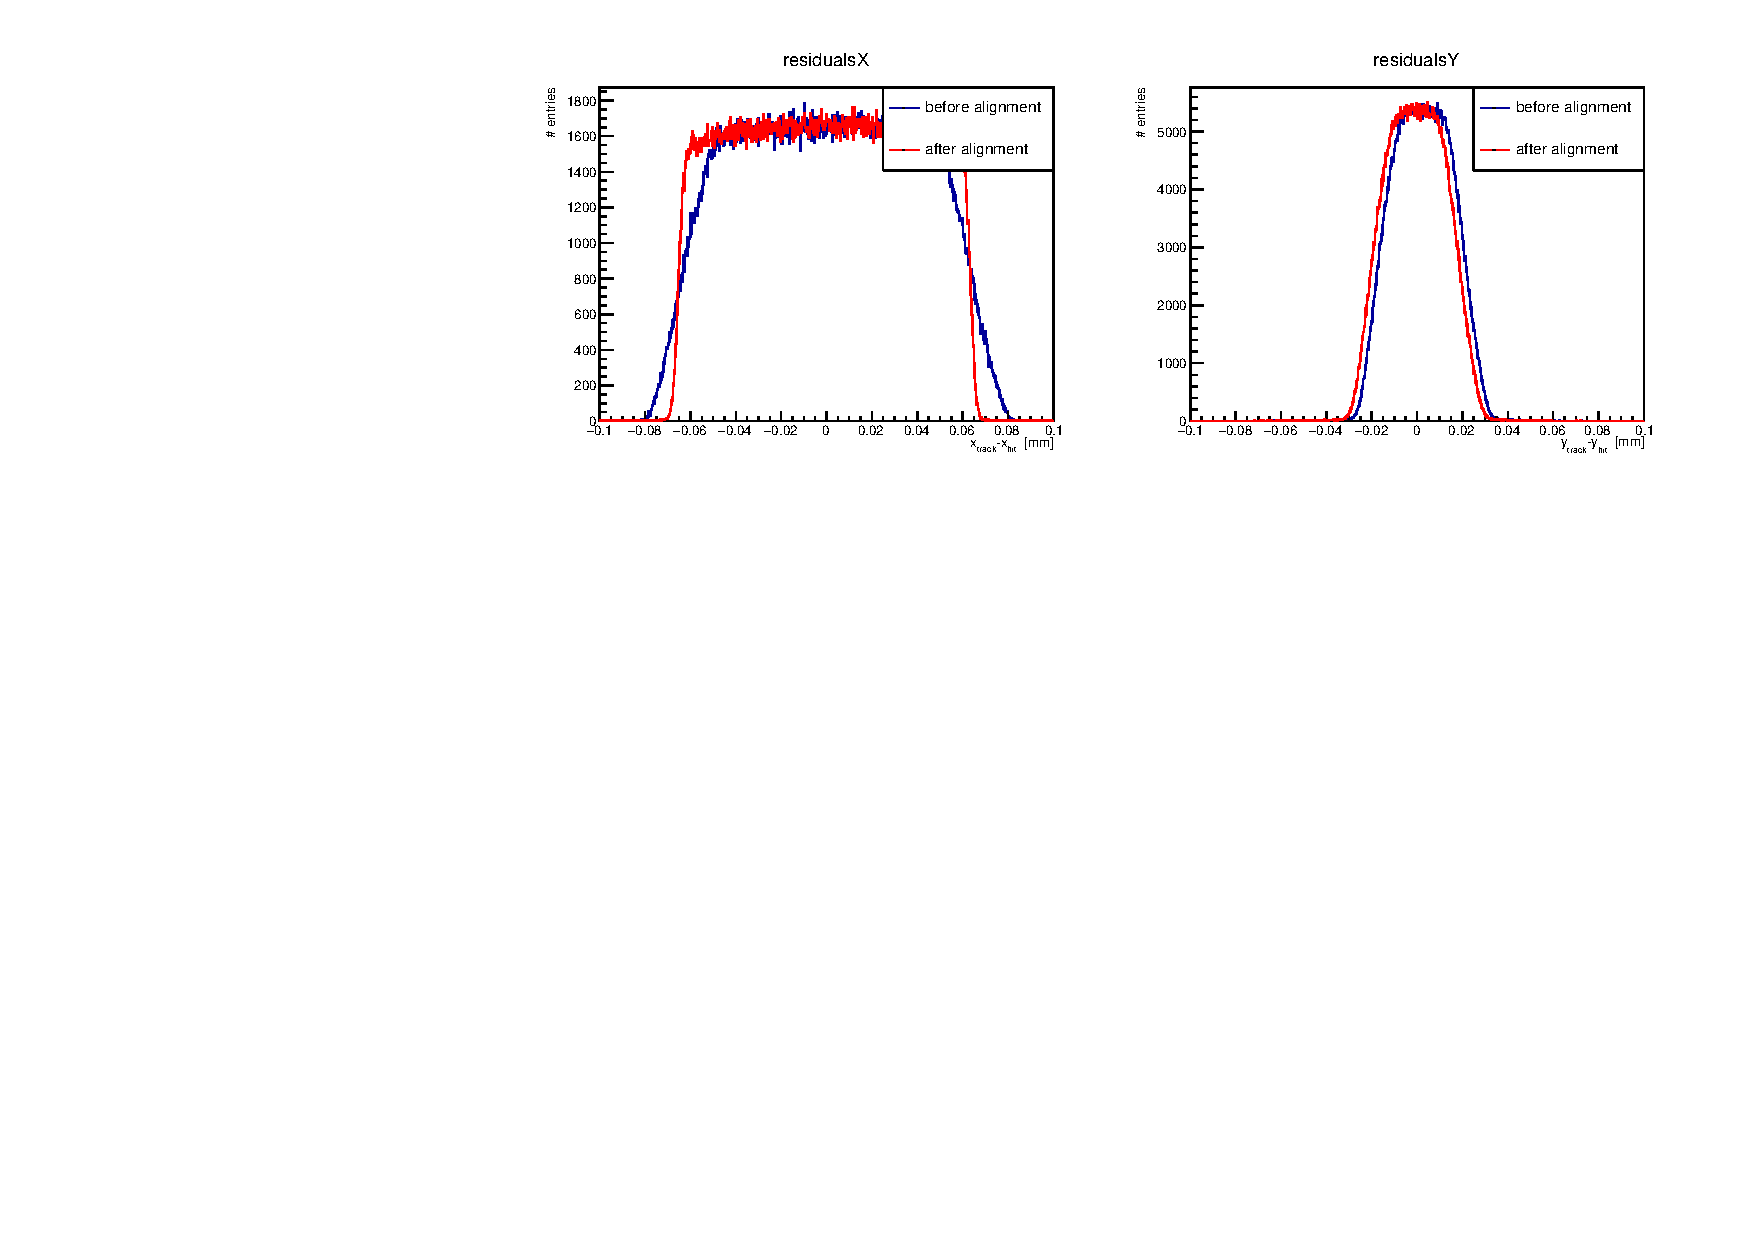
\includegraphics[width=\textwidth]{08_dut_alignment}
\caption{Spatial residuals for the \apx before and after performing the DUT alignment.}
\label{fig:08_dut_alignment}
\end{figure}

\clearpage
\subsection{DUT Analysis}
\textbf{Note:} The entire run is about \SI{470}{s} long:\\ \code{Ev: 23.49M Px: 163.77M Tr: 4.12M (0.175/ev) t = 469.71s}

On the CIP-Pool PC, this is running more than \SI{1}{h}.
In addition, it someimtes to seg faults after \SI{\sim18}{} events.
This seems to be related to the occupancy of the CIP resources.
As a workaround, suggest to the students to limit the analysis by using
\begin{verbatim}
corry -c <config> -o number_of_events=15000000
\end{verbatim}

See Figure~\ref{fig:09_DUTanalysis}.
\begin{itemize}
\item \textbf{In one case, not the entire matrix is filled. Can you explain why? Think about the geometrical dimensions of the \tpx sensors and the \apx.}\\
The \apx sensor is larger than the surface of the \tpx. Consequently, the telescope cannot cover the DUT completely. The hitmap with associated clusters is not entirely filled because on the lower section there are not tracks that can be reconstructed with the telescope.
\end{itemize}

\begin{figure}[!htb]
\centering
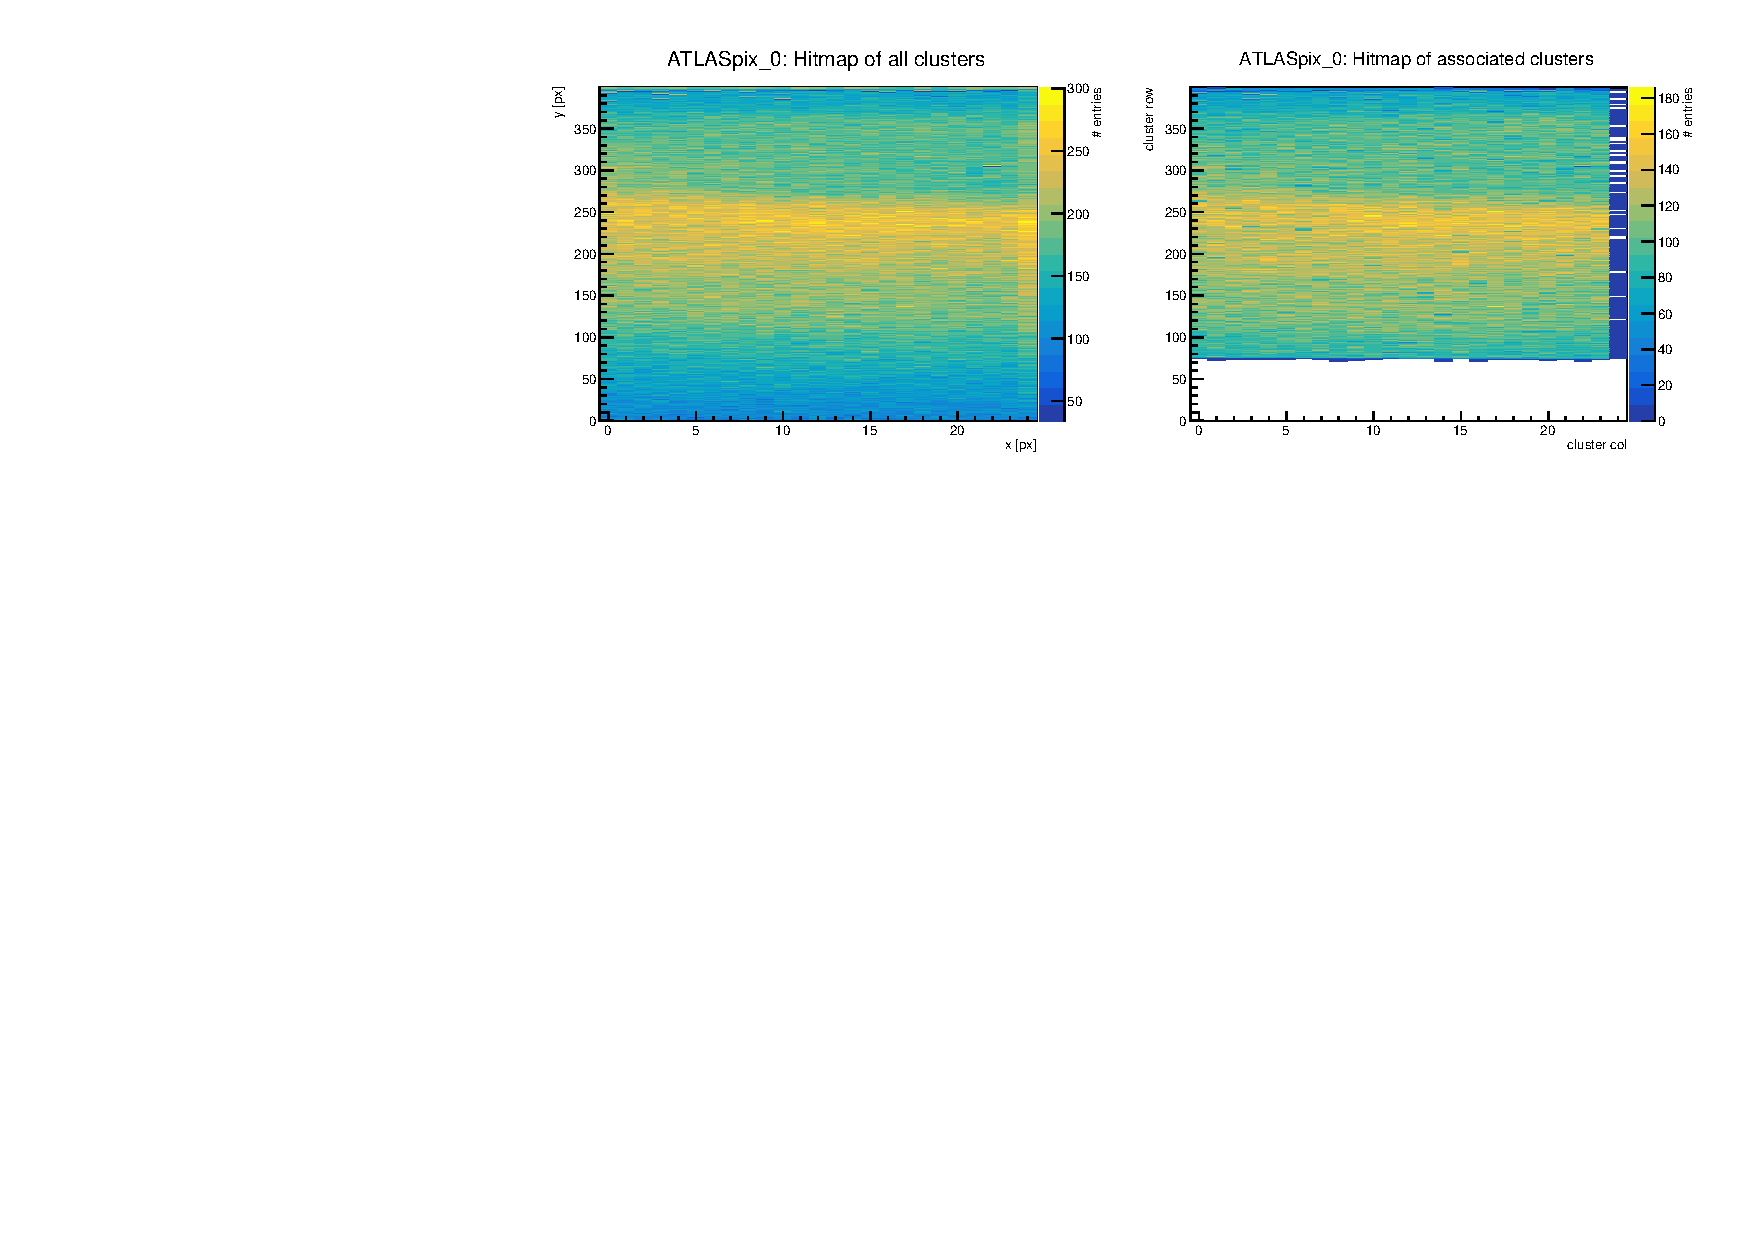
\includegraphics[width=\textwidth]{09_DUTanalysis}
\caption{Hitmaps of all clusters and associated clusters on the \apx.}
\label{fig:09_DUTanalysis}
\end{figure}

\newpage
\subsubsection{Spatial Resolution}
See Figure~\ref{fig:10_spatialResiduals}.

\begin{itemize}
\item \textbf{Are these biased or unbiased residuals? Why?}\\
Here we're looking at unbiased residuals because the \apx hits have been excluded from the tracking.
\item \textbf{Can you quantify the spatial resolutions?} \\
The spatial resolutions can be quantified by looking at the RMS of the spatial distributions. 
We obtain values of \SI{36.9}{\micro m} in the x-direction and \SI{12.9}{\micro m} in the y-direction.
\item \textbf{Are the spatial resolutions what you expected? Why?}\\
The observed spatial resolutions are very close to the \textbf{binary resolution}, which we typed into the geometry file as a first guess at the beginning of the lab course.
The binary resolution is expected if \textbf{only} single-pixel clusters occur. 
This is a good approximation in the case of the \apx.
\item \textbf{Why are the spatial residuals non-gaussian?}\\
The spatial residuals are non-gaussian because of the large pixel pitch of the \apx (\SI{130}{\micro m} and \SI{40}{\micro m}) compared to the tracking resolution of the telescope on the DUT of about \SIrange{1}{2}{\micro m}.
\end{itemize}

\begin{figure}[!htb]
\centering
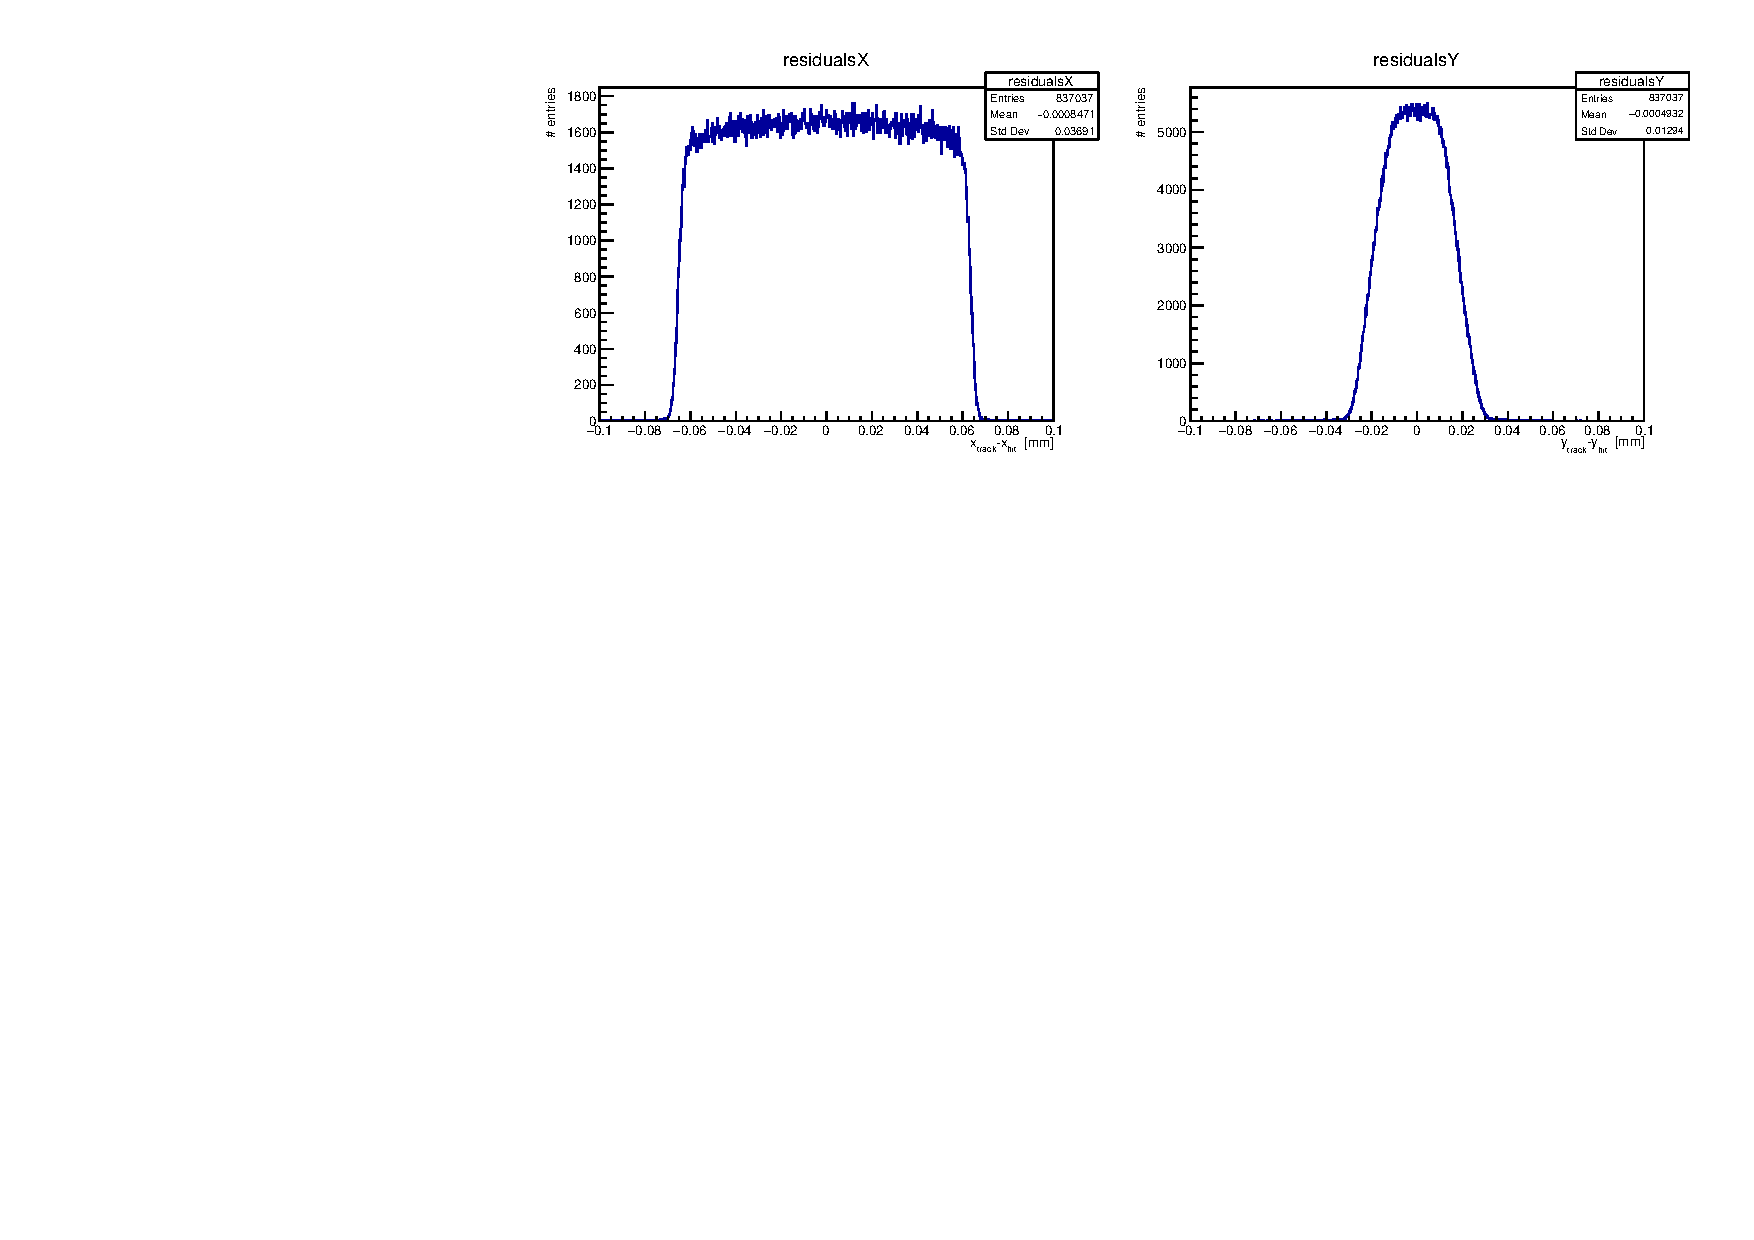
\includegraphics[width=\textwidth]{10_spatialResiduals}
\caption{Spatial residuals in x and y for the \apx.}
\label{fig:10_spatialResiduals}
\end{figure}

\subsubsection{Time Resolution}
See Figure~\ref{fig:11_timeResiduals}.
\begin{itemize}
\item \textbf{Is the peak position (offset from zero) relevant for the time resolution? What may cause it?}\\
The peak position is irrelevant for the timing resolution.
Analogue to the shifts and rotations in space optimised during the alignment, it corresponds to a misalignment in time.
So we could as well add a \code{time\_offset} in the geometry file to correct for it.
It can be caused by differences in signal run-times due to different cable lengths or processing times in the digital periphery of the chip.
\item \textbf{Describe the shape of the distribution and compare it to the 2D histogram. Why is there a strong non-gaussian tail? Does it make sense on which side it is?}\\
The time residual is asymmetric with a tail on the left side.
The left side corresponds to small signals as can be seen in the 2D histogram.
This is the timewalk effect that was discussed in the introduction: small signals have a larger delay than large signals.

\textbf{Note:} The small population at high ToT values is not fully understood yet.
\item \textbf{Can you quantify the time resolution? Compare the Gaussian fit with the RMS of the distribution. Which one is more appropriate?}
The RMS from the statbox of the histogram gives a time resolution of \SI{\sim17}{ns}. In comparison to that, a Gaussian fit yields a $\sigma$ of \SI{\sim13.0}{ns}.
However, the Gaussian fit does not describe the left tail of the distribution.
There is a clear mismatch regarding the left tail.
In addition, the mismatch is reflected in a high $\chi^2/\text{ndf}$ value.
Consequently, the RMS is a better estimation on the time resolution.

\textbf{More precisely:} Quoting a time resolution as a Gaussian $\sigma$ implies that \SI{68}{\percent} of all measurement will deviate from the mean within $\pm1~\sigma$, \SI{95}{\percent} within $\pm2~\sigma$ etc.
This is clearly not the case for the entries in the long tail.

\textbf{Note:} The left tail can be mitigated/removed by applying a timewalk correction.
This makes use of the fact that the peak position of the time residuals depends on the ToT value. 
Hence, a ToT-dependent correction can be applied.
However, this exceeds the scope of this lab course.
\end{itemize}

\begin{figure}[!htb]
\centering
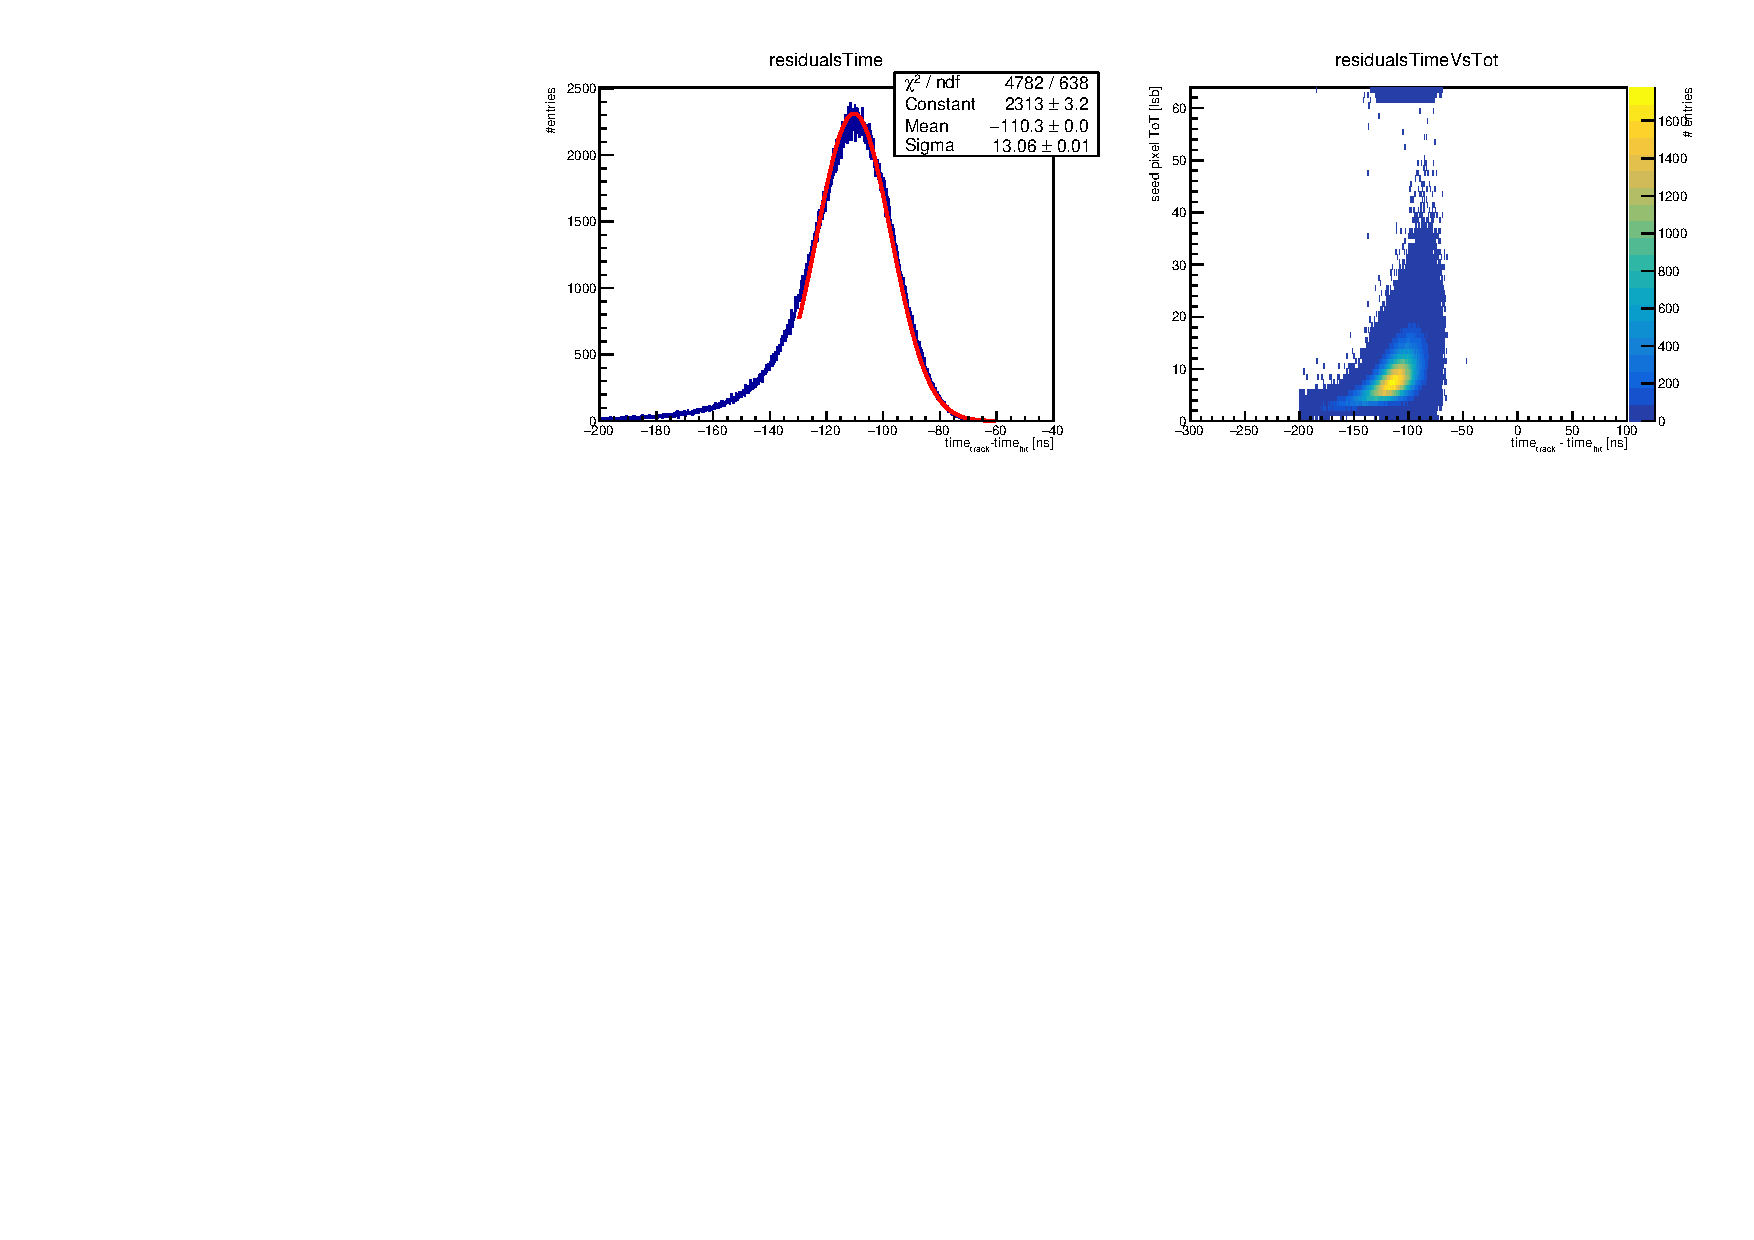
\includegraphics[width=\textwidth]{11_timeResiduals}
\caption{Time residuals in x and y for the \apx.}
\label{fig:11_timeResiduals}
\end{figure}

\subsubsection{Hit Detection Efficiency}
See Figure~\ref{fig:12_efficiency}.
\begin{itemize}
\item \textbf{How large is the hit detection efficiency?}\\
The hit detection efficiency can be read off from the terminal or the \cernroot file in \code{AnalysisEfficiency/ATLASpix\_0/}.
It is about \SI{95.9}{\percent}.
\textbf{Note:} This is not a high efficiency.
The \apx can have an efficiency of more than \SI{99.8}{\percent}. 
The efficiency is low in this data set because it was recorded with a relatively high detection threshold.
This was chosen on purpose such that a stronger effect can be seen in the in-pixel efficiency (see below).
\item \textbf{Why is the chip efficiency map not filled entirely?}\\
The chip efficiency map is not filled entirely for the same reason as above: The \apx cannot be covered completely by the reference telescope because of its larger surface.
Consequently, a second data set with a shifted sensor would need to be analysed to make sure that the sensor is really equally efficient across the entire matrix.
\item \textbf{Do you recognize any pattern in the pixel efficiency map? Can you explain why?}\\
With a good alignment, the telescope resolution is high enough to resolve in-pixel structures.
What can be seen here is that the efficiency drops towards the edges and especially the corners of the pixel.
This is explained by the fact that if a track penetrates the pixel close to its edges it is more likely that charge is shared into the neighbouring cell(s) and the signal amplitude per pixel is smaller.
Therefore, it is more likely that it cannot cross the detection threshold.
\end{itemize}

\textbf{Optional:} 
\begin{itemize}
\item \textbf{Repeat the efficiency analysis multiple times. Systematically scan the spatial cuts in \module{DUTAssociation}.
Plot the measured efficiency versus the association cut.
What do you observe? Can you explain why?}\\
It can be observed that the efficiency starts to drop sharply at some point for smaller and smaller cuts.
This happens at the point where the association cuts are smaller than the spatial resolution of the \apx, i.e.~we start to cut into the spatial residuals.
\end{itemize}

\begin{figure}[!htb]
\centering
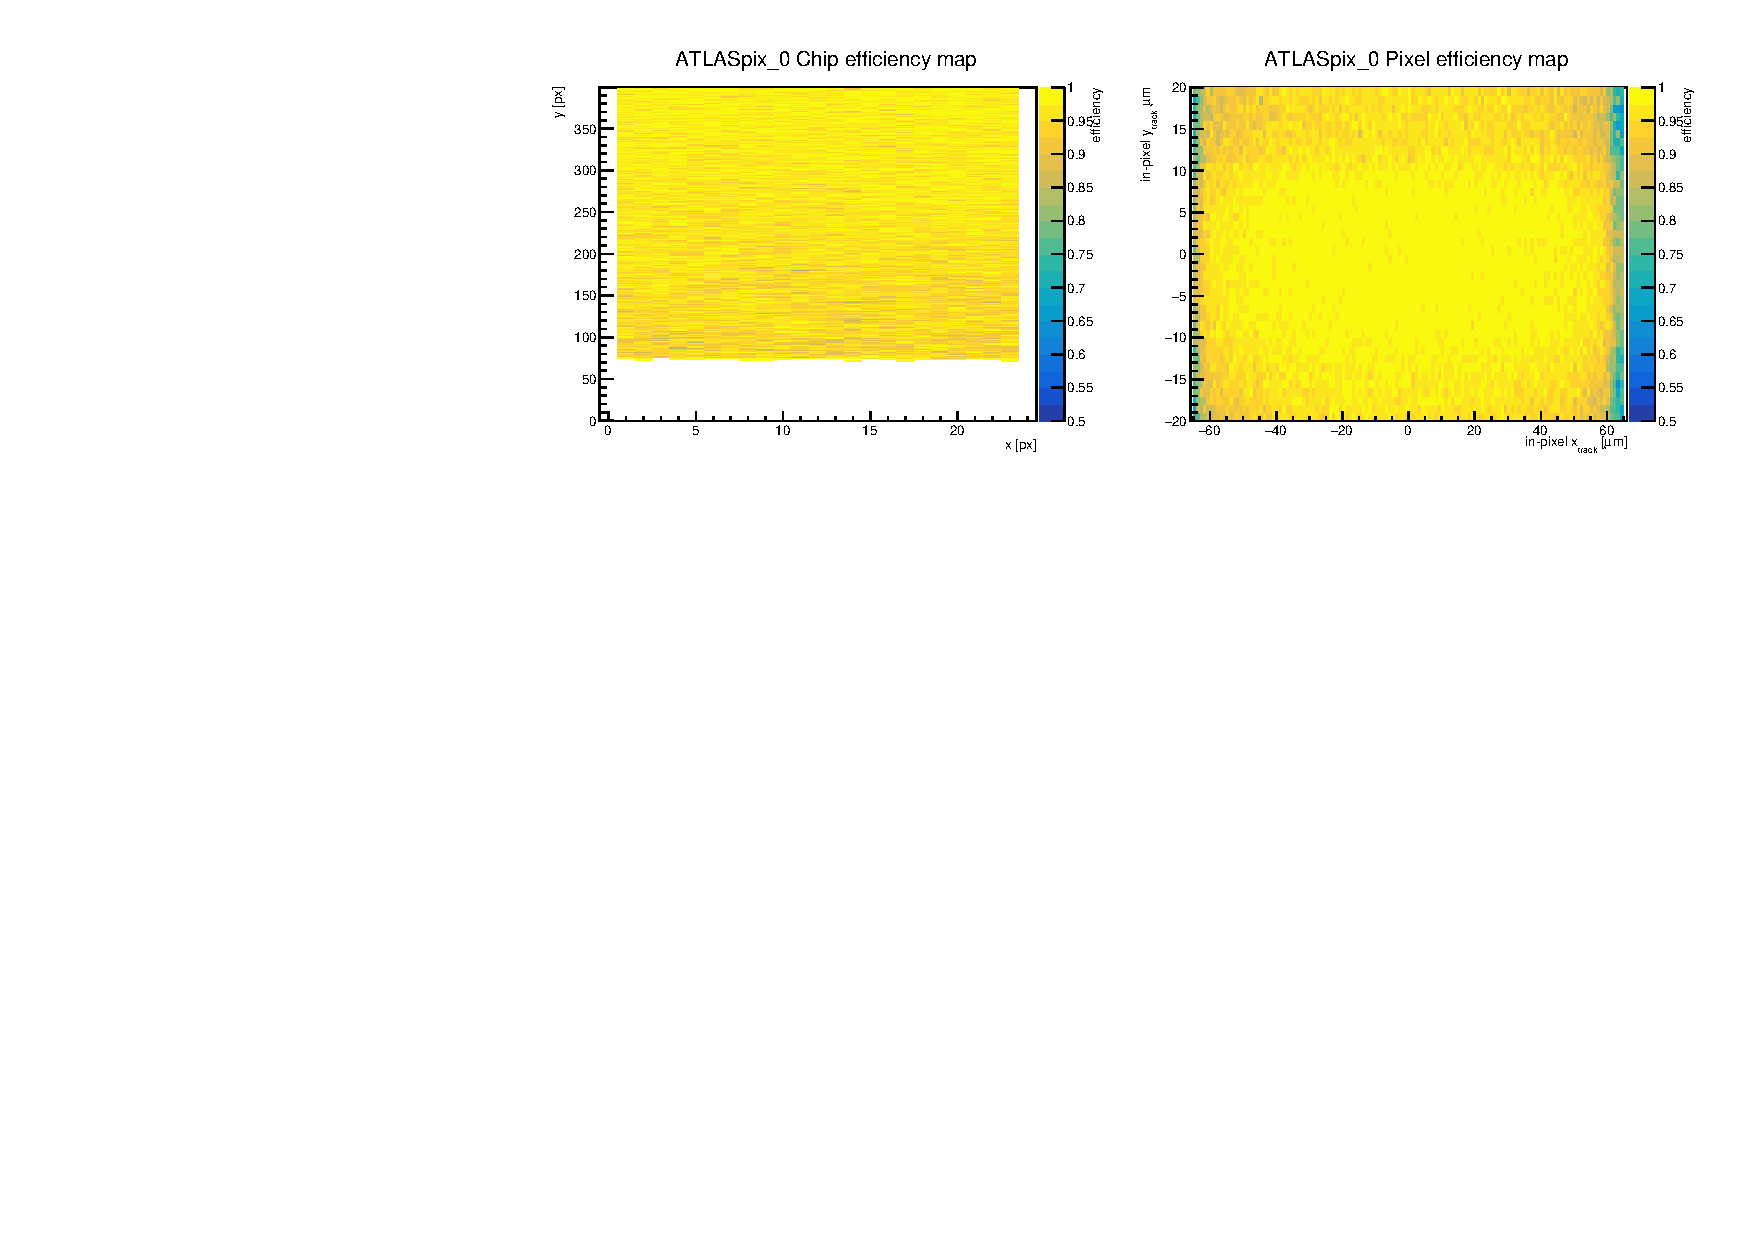
\includegraphics[width=\textwidth]{12_efficiency}
\caption{Hit detection efficiency across the sensor and projected into one pixel cell.}
\label{fig:12_efficiency}
\end{figure}

\section{Closing Remarks}
No questions here.

\end{document}


